\documentclass{article} % For LaTeX2e
\usepackage[final]{colm2026_conference}

\usepackage{microtype}
\usepackage{placeins}
\usepackage{hyperref}
\usepackage{url}
\usepackage{booktabs}
\usepackage{graphicx}
\usepackage{amsmath}
\usepackage{float}
\usepackage{subcaption}

% NOTE: including geometry package
% The geometery package modifies some page properties when used. This can dramatically change the page margins, leading to severe template violation, and potential desk rejection. If the package is required, it can be used with the "pass" flag to skip the default page modifications, as in the following line:
% \usepackage[pass]{geometry}

\usepackage{lineno}

\definecolor{darkblue}{rgb}{0, 0, 0.5}
\hypersetup{colorlinks=true, citecolor=darkblue, linkcolor=darkblue, urlcolor=darkblue}


\title{Latent Linguistic Relations During Diffusion Language Model Denoising}

% CAMERA-READY: the "final" package option above de-anonymizes the paper and
% switches the running head to "Published as a conference paper at COLM 2026".
% The asterisk on the first two authors marks equal contribution.

\author{
Sai Raghuram Jandhyam\thanks{Equal contribution.}, Ryan Dhalbisoi\footnotemark[1], \\
Jennifer Seok, Justice Sefas \\
Algoverse
}

\newcommand{\fix}{\marginpar{FIX}}
\newcommand{\new}{\marginpar{NEW}}

\begin{document}


\maketitle
 
\begin{abstract}
Diffusion language models generate text by iteratively denoising a partially masked sequence, exposing intermediate states that autoregressive models lack. We use these states to ask when, during denoising, a small diffusion model (DiffuGPT-S) forms interpretable linguistic structure, evaluating on held-out natural sentences from the English Web Treebank (UD\_English-EWT). We report three findings. (1)~DiffuGPT-S contains attention heads that track grammatical relations, measured against a fixed-offset baseline tuned exactly as the heads are selected: the strongest object$\to$verb head (L4~H0) predicts the correct receiver with $75.5\%$ held-out accuracy against a $31.4\%$ baseline, and subject$\to$verb also clears its baseline, while the adjective$\to$noun and determiner$\to$noun heads do not---those dependencies are near-adjacent in English and are solved by position alone. Object$\to$verb structure begins to form before full token resolution: $41.6\%$ accuracy while both relation endpoints are still masked, rising to $63.9\%$ once one is revealed---a regime in which no part-of-speech heuristic can operate, because the endpoints have no identity to read. (2)~A depth-wise division of labor: linear probes recover part-of-speech information most accurately from shallow and middle layers, while a logit lens recovers exact token identity far better from deep layers ($40.2\%$ at layer 10 vs.\ $1.2\%$ at layer 0). (3)~Attention structure evolves over diffusion time, with deep-layer heads becoming reliably more selective while shallow layers are heterogeneous.

\end{abstract}

\section{Introduction}

Recent advances in diffusion-based language models 
%suggest that future language models may become increasingly adopt diffusion-style generation, 
suggest that they may become increasingly competitive with autoregressive language models, making it important to understand how these models build linguistic structure during denoising. Unlike autoregressive models, diffusion language models generate text by denoising over time rather than left-to-right. Because many positions remain masked at intermediate steps, they offer a useful interpretability setting: we can ask whether linguistic structure begins to form before the relevant tokens are actually revealed. We study this question in DiffuGPT-S, a small diffusion language model adapted from GPT-2~\citep{gong2025scaling}.

Our analysis builds on attention studies of BERT, where individual heads track positional and linguistic relations~\citep{clark-etal-2019-bert,tenney-etal-2019-bert}, and on recent work on attention sinks and attention floating in diffusion language models~\citep{DBLP:journals/corr/abs-2510-15731,dai2026revealingattentionfloatingmechanism}. In contrast to that prior diffusion-LM work, we focus on which linguistic relations attention heads represent, when these relations appear during denoising, and whether the relevant heads contribute to predicting the eventual masked token or its grammatical class.

We make three main findings. First, DiffuGPT-S contains attention heads that track grammatical relations in natural sentences. Using $1{,}000$ training and $200$ held-out sentences from UD\_English-EWT, we extract subject, object, adjective and determiner dependencies from gold annotations and test whether each head predicts the correct grammatical receiver. The strongest object$\to$verb head reaches $82.9\%$ train and $75.5\%$ held-out accuracy over $220$ instances, and that structure is already partially present while both endpoints remain masked ($41.6\%$, rising to $63.9\%$ once one endpoint is revealed). Subject$\to$verb clears its baseline more narrowly; the adjective$\to$noun and determiner$\to$noun heads score highly in absolute terms but not above a fixed-offset predictor, whose endpoints are adjacent in almost every English instance, so we do not claim them as relation heads.

Second, linear-probe and logit-lens experiments suggest a depth-wise division of labor: shallow and middle layers carry more linearly decodable token-class information, deeper layers more accurate exact-token identity. Direct logit attribution and matched ablations give preliminary evidence that relation heads write relation-specific support for the masked target, but over three head--sentence cases rather than the full evaluation set, so we treat it as suggestive rather than established. Third, attention structure evolves across diffusion time: deeper heads become reliably more selective, while Layer~0 contains heads that become substantially more diffuse. Together these results suggest that masked positions are not inert placeholders---during denoising they participate in partial grammatical structure before their token identities resolve, making the temporal dimension of diffusion models a useful axis for mechanistic interpretability.



\section{Related Work}
\paragraph{Diffusion Language Models}
Diffusion language models (DLMs) are a recent alternative to autoregressive LLMs \citep{brownLanguageModelsAre2020,touvronLLaMAOpenEfficient2023} that generate all positions in parallel and refine them through iterative denoising, providing bidirectional context and BERT-like infilling \citep{liSurveyDiffusionLanguage2025,devlinBERTPretrainingDeep2019} at the cost of multiple forward passes. Most DLMs are discrete: \citet{louDiscreteDiffusionModeling2024} train with a score-entropy objective, while ~\citep{sahooSimpleEffectiveMasked2024}, Dream \citep{yeDream7BDiffusion2025}, and LLaDA \citep{nieLargeLanguageDiffusion} develop masked or diffusion language-modeling objectives for text generation. At inference, masked tokens are revealed in a chosen order---e.g.\ randomly \citep{austinStructuredDenoisingDiffusion2023}, by minimum entropy \citep{yeDream7BDiffusion2025}, or by top-$k$ margin \citep{kimTrainWorstPlan}.


\paragraph{Attention Sinks in Diffusion Language Models}
\citet{DBLP:journals/corr/abs-2510-15731} were the first to explore attention sinks in masked diffusion models. In contrast to autoregressive models, where attention sinks have been observed at beginning-of-sequence or other structural tokens~\citep{xiaoEfficientStreamingLanguage2024,darcetVisionTransformersNeed2024,guWhenAttentionSink2025}, DLMs spread out attention across multiple tokens due to the non-sequential, bidirectional nature of the denoising process and are robust to performance degradations when the sinks are masked. \citet{dai2026revealingattentionfloatingmechanism} further explore this phenomenon, which they call ``attention floating,'' and find that the tokens which receive the most attention are typically structural tokens, e.g.\ punctuation and formatting, which act as guideposts that anchor local context. By rewriting the attention input as a dot product they analyze which layers attend to these structural tokens, finding that shallow layers explore global information, intermediate layers attend to structural patterns, and the deepest layers attend to finer semantic content within that structure. Our work does not look at attention sinks but instead on the linguistic relations that attention heads represent as well as what information attention heads write to the residual stream.

%\paragraph{BERT}
%BERT \citep{devlinBERTPretrainingDeep2019} is a bidirectional language model that predicts masked tokens using left and right context. Two prior works serve as inspiration for our analysis: \citet{clark-etal-2019-bert} investigate which linguistic relations are present in the attention heads of BERT and \citet{tenney-etal-2019-bert} demonstrate that linguistic patterns are processed in a particular order where syntactic roles are processed in the shallow layers and semantic roles are processed in the deeper layers. We find similar results in DiffuGPT-S. In particular, we find object--verb and adjective--noun linguistic relations in its attention heads, and we find that shallow layers process part-of-speech tags whereas deeper layers are responsible for final token prediction. In addition, we extend this analysis in a novel direction by showing that even masked tokens play a role in the linguistic relations found in the attention heads. Specifically, before a token is unmasked, it begins attending to another token in accordance with the linguistic role that the pair will ultimately satisfy at the end of the diffusion process.

\section{Background}
\paragraph{DiffuGPT-S}
DiffuGPT-S is a diffusion language model adapted from GPT-2 small as part of the DiffuGPT family ~\citep{gong2025scaling}. At time $s$ with $0\le s<t\le 1$, it performs inference in continuous time given a sequence of tokens by first predicting $x_0$, the sequence of final unmasked tokens, and then sampling from the following posterior 
\[ q(x_s \mid x_t, x_0) =\begin{cases}
      \frac{\alpha_s-\alpha_t}{1-\alpha_t}x_0+\frac{1-\alpha_s}{1-\alpha_t}m & x_t=m \\
      x_0 & x_t\ne m \text{,}\\
   \end{cases}
\]
where $m$ denotes a special masked token and $\alpha_s, \alpha_t$ are hyperparameters defined by the noise schedule.

\paragraph{Attention}
Each layer of DiffuGPT-S contains a self-attention sublayer with $H=12$ heads followed by a fully connected sublayer. Head $h$ in layer $\ell$ computes $A^{\ell,h}=\mathrm{softmax}\!\left(Q_hK_h^{\top}/\sqrt{d_{model}}\right)V_h$ from learned projections of the input, and the heads are concatenated and mixed by a learned output matrix $W^O$ to form the layer's attention output $\mathbf{a}^\ell$. We use bold $\mathbf{a}^{\ell}$ for that output to distinguish it from the layer representations $a_i^\ell(t)$ used in the probing experiments (Section~\ref{subsec:probes}).

\section{Methodology}\label{sec:methodology}
\subsection{Direct Logit Attribution}\label{subsec:dta}
We use Direct Logit Attribution (DLA), a per-head logit lens \citep{nostalgebraist2020logitlens}, which isolates the additive contribution of a single attention head to the residual stream by projecting it into vocabulary space through the model's unembedding.

For layer $\ell$, head $h$ and position $i$, the attention sublayer forms the value-weighted context $o^{\ell,h}_i\in\mathbb{R}^{d_h}$. Because the output projection $W_O^\ell$ acts linearly on the concatenated heads, the attention write decomposes exactly into per-head terms $c^{\ell,h}_i = o^{\ell,h}_i\,W_O^{\ell,(h)}$, which we project through the final norm $\mathrm{LN}_f$ and unembedding $W_U$:
\begin{equation}
  z^{\ell,h}_i = W_U\,\mathrm{LN}_f\!\big(c^{\ell,h}_i\big)\in\mathbb{R}^{|V|}.
\end{equation}
Let $p$ be the target position and $w^\star$ its ground-truth token. We summarize a head's support for $w^\star$ by the vocabulary percentile $\pi^{\ell,h}=1-(r^{\ell,h}-1)/|V|$ of its rank $r^{\ell,h}$ under $z^{\ell,h}_p$; a value near $1$ indicates strong exact-token support. To separate grammatical from lexical support we also compute a token-type attribution $\bar{\phi}^{\ell,h}_{G}=\tfrac{1}{|G|}\sum_{w\in G} z^{\ell,h}_p[w]$ over a set $G$ of tokens sharing $w^\star$'s syntactic category.

We evaluate DLA at a chosen timestep on a masked target position and rank all $L\times H$ heads by $\pi^{\ell,h}$ and $\bar{\phi}^{\ell,h}_{G}$, distinguishing genuinely token-predictive heads from those that merely attend to the relevant position. DLA is correlational; we pair it with causal head ablation (Appendix~\ref{app:relation_heads}, Table~\ref{tab:mini_control_ablation}), which zeroes $c^{\ell,h}_p$ and measures the induced change in the same quantities.



\subsection{Linear Probes}\label{subsec:probes}
To measure how much part-of-speech (POS)/token-class information is linearly decodable at different depths, we train linear probes on the model's internal representations. The representation for token $i$ at layer $\ell$ and diffusion step $t$ is $a_i^\ell(t)\in\mathbb{R}^{d}$; DiffuGPT-S is frozen, so probe accuracy reflects only information already readable from its denoising representations. For each probed layer we train a linear classifier over the token-class label set $\mathcal{Y}$, $\hat{y}_i^\ell(t)=\arg\max_{y\in\mathcal{Y}}\mathrm{softmax}(W_p^{(\ell)}a_i^\ell(t)+b_p^{(\ell)})_y$.


Gold POS labels are obtained by running the Stanford log-linear part-of-speech tagger~\citep{toutanova2003featurerich} on the fully unmasked final sentence. The tagger labels based on the POS label set:

\[
\mathcal{Y}=\{\mathrm{NOUN}, \mathrm{VERB}, \mathrm{ADJ}, \mathrm{ADV}, \mathrm{PREP}, \mathrm{DET}, \mathrm{PRON}, \mathrm{CONJ}\}.
\]

Word-level POS tags and DiffuGPT-S subword tokens are aligned using tokenizer offsets. Subwords receive the POS tag of the original word, and special tokens and tags outside the selected label set are excluded.

Separate probes are trained for layers \(\ell \in \{2,5,10\}\), representing shallow, middle, and deep layers. The probes are trained on $1{,}000$ sentences and evaluated on $200$ held-out sentences, with no sentence overlap between the two datasets. Because our main focus is understanding whether grammatical-category information is available before token identity is revealed, we focus especially on masked-token positions during denoising.

To validate probe accuracy, we compare against a majority-class baseline, shuffled-label probes, and random-feature probes with the same dimensionality. Linear probes show whether POS information is readable from the representation; they do not by themselves prove causal use.

\subsection{Relation-Head Receiver Prediction}

To test whether individual attention heads track grammatical relations, we define a receiver-prediction task over gold dependency annotations. Unlike the POS probes in Section 4.2, which measure whether token-class information is linearly decodable from hidden states, this experiment evaluates whether an attention head routes attention from one grammatical token to another. We use 1,000 training sentences and 200 held-out evaluation sentences drawn from the English Web Treebank (UD\_English-EWT), a human-annotated Universal Dependencies corpus \citep{nivre2020universal}. Sentences are taken in corpus order from the treebank's training and development files. For each sentence, we extract directed dependency instances $e=(a,r,\rho)$, where $a$ is the attender word, $r$ is the receiver word, and $\rho$ is the relation type. We include object$\rightarrow$verb, subject$\rightarrow$verb, adjective$\rightarrow$noun, and determiner$\rightarrow$noun relations, corresponding to UD dependency labels such as \texttt{obj}, \texttt{nsubj}, \texttt{amod}, and \texttt{det}.

Because dependency annotations are word-level while DiffuGPT-S operates on byte pair encoding (BPE) subword tokens, we align each UD word to a DiffuGPT-S token span using tokenizer character offsets, following the same word-to-subword alignment principle used for POS labels in Section 4.2. Let $S(w)$ denote the BPE token span aligned to word $w$. We discard a dependency instance if either $S(a)$ or $S(r)$ is empty.

For a layer $\ell$, head $h$, timestep $t$ and instance $e=(a,r,\rho)$, we aggregate the attention sent from the attender span to each candidate source token $j$ as $s^{\ell,h}_{j}(e,t)=\lvert S(a)\rvert^{-1}\sum_{i\in S(a)} A^{\ell,h}_{ij}(t)$. Excluding the beginning-of-sequence (BOS) token and the attender's own span from the candidate set, the head's predicted receiver is $\hat{j}^{\ell,h}(e,t)=\arg\max_{j \notin S(a)\cup\{\mathrm{BOS}\}} s^{\ell,h}_{j}(e,t)$, and a prediction counts as correct when $\hat{j}^{\ell,h}(e,t)\in S(r)$.

For each relation type $\rho$, receiver-prediction accuracy is the mean of this indicator over all gold dependency instances of that type. We score all layer--head pairs on the 1,000-sentence training split and select the highest-scoring head for each relation type. We then report the selected head's accuracy on the 200-sentence held-out split. 

Because a head that always attends a fixed number of positions from itself would solve any dependency whose endpoints sit at a near-constant distance, we compare each selected head against a fixed-offset predictor. For relation $\rho$ we choose the single offset
\begin{equation}
k^\star_\rho=\arg\max_{k\neq 0}\ \frac{1}{|E^{\mathrm{train}}_\rho|}\sum_{e\in E^{\mathrm{train}}_\rho}\mathbf{1}\!\left[\max S(a)+k \in S(r)\right],
\end{equation}
fit on the same training split used to rank heads, and report its accuracy on the held-out split. The offset $k=0$ is excluded because the attender's own span is removed from the head's candidate set, so the baseline may not predict it either. This baseline receives exactly the tuning the head does, which the random and nearest-token controls do not: a nearest-token rule that breaks ties toward the preceding token scores $0.000$ on determiner$\to$noun, where the receiver is always the following word, and so understates how much position alone explains. We report Wilson score intervals on held-out head accuracy and treat a relation as evidenced only when that interval lies entirely above the fixed-offset baseline.


To test whether relation structure appears before token resolution, we also evaluate the selected heads across diffusion timesteps. For each timestep, we split dependency instances according to whether both endpoint spans $S(a)$ and $S(r)$ are still masked. Masked-state accuracy is receiver-prediction accuracy restricted to instances where both endpoints remain masked, while unmasked accuracy is computed over instances where at least one endpoint has been revealed. This separates relation structure that is available during denoising from relation structure that appears only after the relevant tokens become visible.



\subsection{Metric Definitions}\label{subsec:metrics}

The sharpness of attention head $h$ in layer $\ell$ at diffusion time $t$ is
measured by the entropy of each query token's attention distribution,
$H^{\ell,h}_i(t) = -\sum_{j=1}^{S} A^{\ell,h}_{ij}(t)\log A^{\ell,h}_{ij}(t)$,
where lower values indicate attention concentrated on fewer source tokens. We also report the per-layer mean over heads,
$\bar{H}^{\ell}_i(t)=\tfrac{1}{H}\sum_h H^{\ell,h}_i(t)$.

For a head's support of the eventual token we use the exact-token vocabulary
percentile $\pi^{\ell,h}$ and the token-type attribution $\bar{\phi}^{\ell,h}_G$; a percentile near $1$ indicates the head
ranks the correct token near the top of the vocabulary.

For relation-head experiments, receiver-prediction accuracy is the fraction of gold dependency instances for which a head's max-attended source token from the attender span falls inside the gold receiver's BPE token span, excluding the BOS token and the attender span itself. In timestep-resolved analyses, masked-state accuracy is computed only over instances where both endpoint spans remain masked at timestep $t$, while unmasked accuracy is computed over instances where at least one endpoint span has been revealed. In relation-head tables, eval $n$ denotes the number of gold dependency instances in the held-out evaluation split, not the number of sentences.




\section{Attention}
\subsection{Attention Entropy}

We first measure whether attention becomes more diffuse or more selective over diffusion time using the entropy metric defined in Section~4.4. Higher entropy indicates attention spread across more source positions, while lower entropy indicates more concentrated attention.

\begin{table}[H]
\centering
\small
\begin{tabular}{lrrrrrrr}
\toprule
Layer & Heads & $H_{\mathrm{early}}$ & $H_{\mathrm{late}}$ & Median $\Delta H$ & \% inc. & \% dec. & \% flat \\
\midrule
0  & 12 & 0.624 & 0.643 & -0.002 & 41.7 & 41.7 & 16.7 \\
10 & 12 & 0.463 & 0.300 & -0.200 & 16.7 & 83.3 & 0.0 \\
\bottomrule
\end{tabular}
\caption{Entropy-change summary across attention heads in representative shallow and deep layers. $H_{\mathrm{early}}$ and $H_{\mathrm{late}}$ denote normalized attention entropy averaged over query tokens, sentences, and early/late diffusion windows. We define $\Delta H = H_{\mathrm{late}} - H_{\mathrm{early}}$, so positive values indicate that attention becomes more diffuse over denoising, while negative values indicate that attention becomes more concentrated. The columns \% inc., \% dec., and \% flat report the fraction of heads in the layer with $\Delta H > 0.02$, $\Delta H < -0.02$, and $|\Delta H| \leq 0.02$, respectively.}
\label{tab:entropy_summary}
\end{table}

Table~\ref{tab:entropy_summary} shows that Layer~10 attention becomes more selective over denoising: $83.3\%$ of Layer~10 heads decrease in entropy, with median $\Delta H=-0.200$. Layer~0 is more heterogeneous, with equal fractions of increasing and decreasing heads, though some heads such as L0~H0, L0~H2, and L0~H4 become strongly more diffuse. Representative heatmaps for these two behaviors are shown in Appendix~\ref{app:entropy_heatmaps}.

\subsection{Attention Pattern Evolution}\label{subsec:attn_patterns}

In the next set of experiments, we analyze the linguistic relations found in the attention heads and investigate how they evolve during the unmasking process. Attention heatmaps for the final unmasked sequence reveal standard positional patterns---current-token, next-token, previous-token, and stop-word heads---as well as BERT-style linguistic relations \citep{clark-etal-2019-bert} including verb--object, adjective--noun, and subject--verb heads (Appendix~\ref{app:attention_patterns}, Figure~\ref{fig:all_heads}). Figure~\ref{fig:object-verb} (Appendix~\ref{app:attention_patterns}) shows L2~H8 as a qualitative object$\to$verb example.

As a qualitative illustration, we inspected a small set of diagnostic sentences with known relations, e.g.\ the object--verb relation in ``The student considered the problem extremely difficult.'' L2~H8 provides a qualitative diagnostic example of object$\to$verb attention at masked timesteps (Figure~\ref{fig:object-verb}); the held-out UD timestep analysis below provides the quantitative test across diffusion time.

To move beyond hand-picked stimuli, we search for relation heads on natural sentences from the English Web Treebank (UD\_English-EWT) \citep{nivre2020universal}: $1{,}000$ training and $200$ held-out sentences with gold subject$\to$verb, object$\to$verb, adjective$\to$noun, and determiner$\to$noun pairs. For each head we predict the receiver as the source token the attender attends to most (excluding the \texttt{BOS} sink and the attender's own position), rank heads on the training split, and report held-out accuracy against simple heuristic baselines (Table~\ref{tab:relation_baselines}). Random attention is not the relevant null: in English the endpoints of adjective$\to$noun and determiner$\to$noun dependencies are adjacent almost by construction, so a head that always attends a fixed number of positions away solves them without representing any syntax. We therefore compare each head against Offset$^\star$, the best single fixed offset $\hat{r}=a+k$, with $k$ fit on the training split and evaluated held-out so the baseline receives exactly the tuning the head does. Two relations clear it: object$\to$verb ($0.755$ vs.\ $0.314$) and subject$\to$verb ($0.521$ vs.\ $0.429$). For the noun-modifier relations the Wilson interval contains the offset baseline, and for subject determiner$\to$noun the baseline is higher; we do not claim these heads encode those relations. The oracle nearest-POS baseline is higher still on every row, bounding how much of the final-step signal locality plus POS regularity explains. Crucially that oracle cannot run during denoising---it must read parts of speech that are undefined while the endpoints are masked---so the masked-state analysis below is not subject to it. Object$\to$verb is the one relation no fixed offset and no POS-locality heuristic solves, and we treat it as the paper's central case.

%To move beyond hand-picked stimuli, we search for relation heads on natural sentences from a gold Universal Dependencies treebank \citep{nivre2020universal}: $1{,}000$ training and $200$ held-out sentences with gold subject$\to$verb, object$\to$verb, adjective$\to$noun, and determiner$\to$noun pairs. For each head we predict the receiver as the source token the attender attends to most (excluding the \texttt{BOS} sink and the attender's own position), rank heads on the training split, and report held-out accuracy against non-neural baselines (Table~\ref{tab:ud_relation_heads}). The strongest object$\to$verb head, \textbf{L4~H0}, reaches $75.5\%$ held-out receiver-prediction accuracy ($220$ instances); adjective$\to$noun and determiner$\to$noun heads also transfer, whereas subject$\to$verb transfer is weak.

To test whether these relations appear before the tokens are resolved, we evaluate the selected heads at every diffusion timestep on the held-out set, splitting instances by whether both relation endpoints remain masked (Figure~\ref{fig:ud_relation_accuracy_over_time}). The object$\to$verb head L4~H0 predicts the correct receiver with $41.6\%$ accuracy while both endpoints are still masked---above its $30.9\%$ at full masking and far above chance---rising to $63.9\%$ once at least one endpoint is revealed and $75.5\%$ on the fully unmasked sentence. Object--verb structure is therefore partially present during denoising, before full token resolution, rather than appearing only at the end.

\begin{table}[t]
\centering
\footnotesize
\setlength{\tabcolsep}{3pt}
\renewcommand{\arraystretch}{1.08}
\begin{tabular*}{\textwidth}{@{\extracolsep{\fill}}llrrrrrr}
\toprule
Relation & Top head & Head (95\% CI) & Random & Offset$^\star$ & Oracle POS & Wrong POS & $n$ \\
\midrule
Object $\to$ verb & L4 H0 & \textbf{0.755} {\scriptsize[.694,.807]} & 0.061 & 0.314 & 0.845 & 0.011 & 220 \\
Subject $\to$ verb & L6 H1 & \textbf{0.521} {\scriptsize[.465,.577]} & 0.059 & 0.429 & 0.581 & 0.067 & 303 \\
Obj. adj. $\to$ noun & L6 H1 & 0.827 {\scriptsize[.703,.906]} & 0.041 & 0.750 & 0.923 & 0.006 & 52 \\
Subj. adj. $\to$ noun & L0 H3 & 0.682 {\scriptsize[.534,.800]} & 0.047 & 0.682 & 0.841 & 0.023 & 44 \\
Obj. det. $\to$ noun & L4 H3 & 0.600 {\scriptsize[.494,.698]} & 0.057 & 0.553 & 0.765 & 0.022 & 85 \\
Subj. det. $\to$ noun & L4 H3 & 0.589 {\scriptsize[.486,.685]} & 0.052 & 0.600 & 0.789 & 0.036 & 90 \\
\bottomrule
\end{tabular*}
\caption{Held-out receiver-prediction accuracy for selected UD relation heads, with Wilson score intervals. Random chooses a valid non-BOS, non-self token. Offset$^\star$ is the best fixed-offset predictor $\hat{r}=a+k$, with $k$ chosen on the training split and reported held-out, so the baseline is tuned exactly as the head is selected ($k=-2$ for object$\to$verb, $k=+1$ otherwise). Oracle POS chooses the closest token carrying the gold receiver's POS tag, and is an oracle in that it reads parts of speech the model cannot access while endpoints are masked. Wrong POS scores the same predictions against incorrect same-POS receivers. Bold marks the relations whose interval clears Offset$^\star$.}

\label{tab:relation_baselines}
\end{table}



% TODO(authors) -- UNRESOLVED BEFORE SUBMISSION.
% Two open items on this figure, both raised by Reviewer hwdx ("thin statistical
% reporting with no confidence intervals or multi-seed aggregates for core numbers"):
%
% 1. The 41.6%% / 63.9%% masked and unmasked numbers reported here appear to come
%    from a single run. A five-seed sweep (seeds 42-46) exists in
%    ud_relation_accuracy_masked_vs_unmasked_seeds.csv and gives 43.4%% +/- 3.3%%
%    masked and 61.7%% +/- 1.9%% unmasked -- close, but NOT the same numbers.
%    Decide which protocol is canonical, rerun if needed, and report mean +/- std
%    over seeds in both the caption and the abstract. Do not ship both.
%
% 2. Once (1) is settled, add the matched fixed-offset baseline to the masked-state
%    comparison: the k*=-2 offset must be evaluated on exactly the instances that
%    enter the masked-state average, not on the whole split.
\begin{figure}[t]
\centering
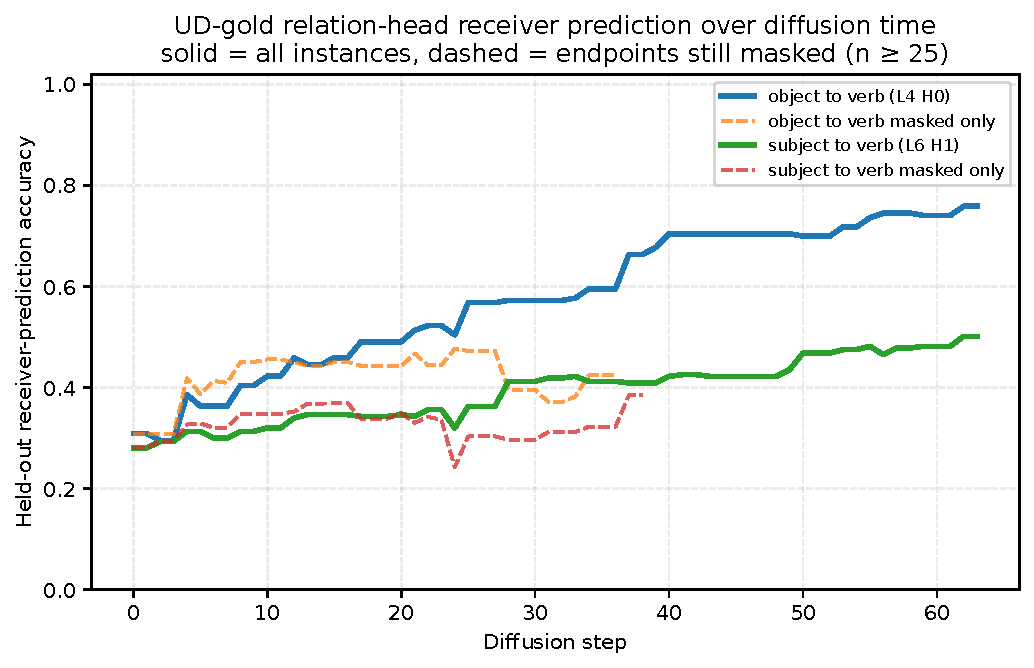
\includegraphics[width=0.66\linewidth]{figures/ud_relation_accuracy_over_diffusion_time_minmasked25.pdf}
\caption{Held-out receiver-prediction accuracy over diffusion time for selected relation heads on natural UD sentences. Solid curves show accuracy over all relation instances at each timestep. Dashed curves show accuracy restricted to instances where both relation endpoints remain masked, and are plotted only when at least 25 masked instances remain. The object$\rightarrow$verb head L4 H0 predicts the correct receiver with 41.6\% masked-state accuracy and 63.9\% unmasked accuracy, indicating that object--verb structure is partially available before full token resolution.}
\label{fig:ud_relation_accuracy_over_time}
\end{figure}


Beyond where these heads attend, direct logit attribution and causal ablation indicate that, on three individually inspected diagnostic sentences, high-relation heads write relation-specific support into the residual stream: ablating these heads---zeroing each head's contribution to the residual stream---lowers the correct target's logit more than ablating low-relation control heads matched on the same sentence, target token, seed, and diffusion timestep (Appendix~\ref{app:relation_heads}, Table~\ref{tab:mini_control_ablation}). 

\subsection{Shallow and Middle Layers Encode Token Class}\label{subsec:shallow_class}

Attention heatmaps show where a head attends, but they do not reveal what information it writes into the residual stream. A head can attend to the correct verb or object without promoting it in the model's output distribution. We therefore ask two questions, testing each with the probes, logit-lens, and DLA readouts described in Section~\ref{sec:methodology}: Do masked positions carry decodable token-class (POS) information? And do they carry decodable exact-token identity?

As shown in Figure~\ref{fig:pos_probe_mask_ratio}, POS information is highly decodable from masked-token representations. Layer~2 and Layer~5 remain strongest across mask ratios: averaged over masked positions, Layer~2 reaches $0.879$ and Layer~5 $0.878$, against $0.783$ for Layer~10. Broad grammatical-category information is therefore available in earlier and middle representations while positions remain masked, before the model resolves exact token identity. Real probes greatly exceed majority-class, shuffled-label and random-feature controls (Appendix~\ref{app:linear_probe_results}, Table~\ref{tab:pos_probe_controls}), and within Layer~2 the strongest heads sit far above the majority baseline while others are near it, so grammatical-category information is not uniformly distributed across heads.

\begin{figure}[t]
\centering
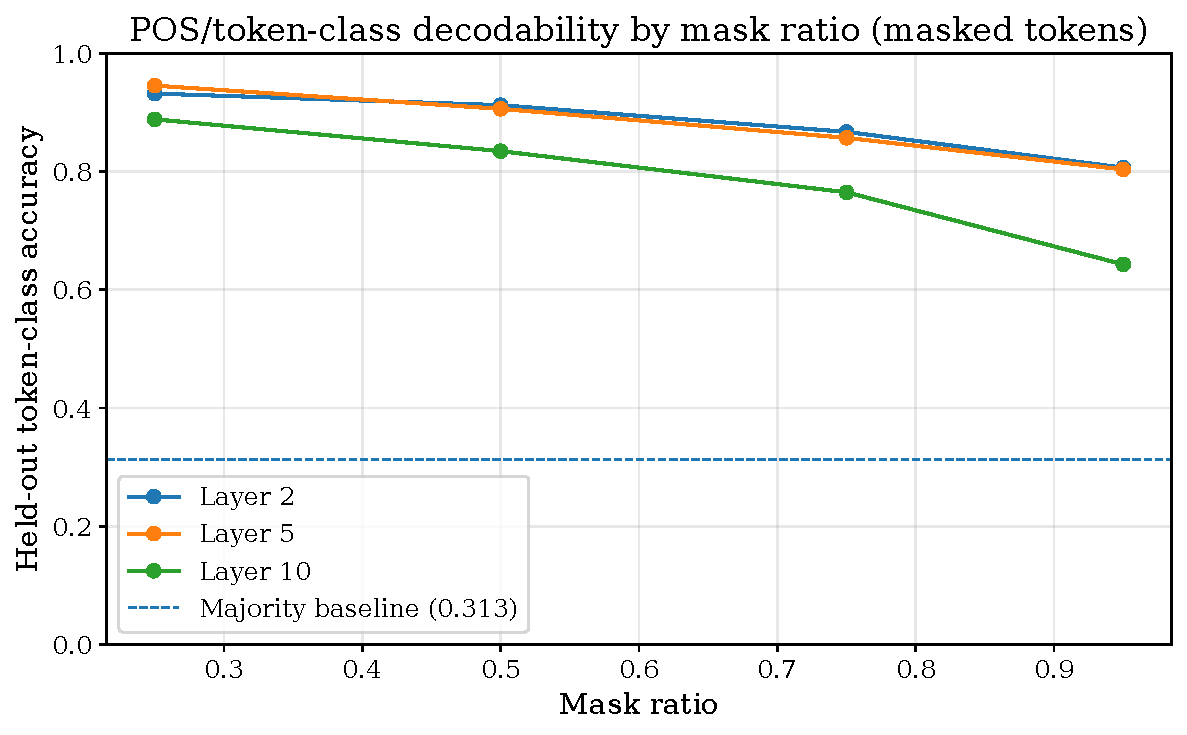
\includegraphics[scale=0.38]{figures/controlled_probe_accuracy_by_mask_ratio_masked.pdf}
\caption{POS/token-class probe accuracy on masked-token positions across mask ratios. Layer~2 and Layer~5 remain highly decodable even at high mask ratios, while Layer~10 performs lower.}
\label{fig:pos_probe_mask_ratio}
\end{figure}

These probes are diagnostic rather than causal. To test causal necessity, we ablate the top POS-decodable heads in each layer and compare the accuracy drop against ablating lower-decoding control heads. Across the three layers, the top-decodable heads do not produce a larger drop than the controls (Appendix~\ref{app:linear_probe_results}, Figure~\ref{fig:pos_ablation_top_minus_control}). High linear decodability does not imply causal necessity; POS information is available in the representation but is distributed rather than concentrated in specific heads.

\subsection{Deeper Layers Encode Future Token Identity}
\label{subsec:deep_identity} 

Section~\ref{subsec:shallow_class} showed that token class is most linearly
decodable in shallow layers; we now ask where token identity is written. For
layers $0$, $5$, and $10$ we apply a logit lens \citep{nostalgebraist2020logitlens} to each layer's residual
representation at still-masked positions---projecting it through the model's final
norm and unembedding (Section~\ref{subsec:dta})---and measure how often the top-1
token equals the eventual unmasked token, averaged over diffusion time
(Figure~\ref{fig:final_token_prediction}). The ordering is the reverse of the
part-of-speech probe: the deepest probed layer (L10) decodes the eventual token
with mean accuracy \textbf{40.2\%}, far above the middle (L5, \textbf{7.6\%}) and
shallow (L0, \textbf{1.2\%}) layers. Token identity is thus written predominantly
in deep layers, while shallow layers carry grammatical class---a depth-wise
division of labor consistent with the syntactic-before-semantic ordering reported
for BERT \citep{tenney-etal-2019-bert}.

This identity information is available before tokens are revealed: the final-layer argmax matches the eventual token a median of seven diffusion steps before unmasking ($63.4\%$ of positions predicted early), with punctuation and function words committed earliest; full timing statistics and the sampling-induced ceiling on this measurement are given in Appendix~\ref{app:timing}. The POS probes locate where grammatical information is available, whereas the logit-lens readout locates where the network begins predicting a particular future token.

\section{Discussion and Conclusion}

DiffuGPT-S develops interpretable attention structure over the course of denoising rather than only at the final step. Attention entropy shifts across diffusion time, and the model shows a depth-wise division of labor in which shallow layers carry token class and deep layers carry exact token identity. Most importantly, object--verb structure begins to form before the tokens resolve: on $200$ held-out UD\_English-EWT sentences the strongest object$\rightarrow$verb head, L4~H0, reaches $75.5\%$ receiver-prediction accuracy over $220$ instances against $31.4\%$ for the best fixed-offset predictor, and still predicts the receiver $41.6\%$ of the time while both endpoints remain masked. Object$\to$verb and subject$\to$verb are the two relations we claim on this basis; the adjective$\to$noun and determiner$\to$noun heads, though accurate, are not separable from position in English. The temporal dimension of denoising is therefore a useful and underexplored axis for mechanistic interpretability.


Our claims are limited. All experiments use DiffuGPT-S, so the specific heads and depth-wise trends may not transfer to larger or differently-trained diffusion models; and because it is initialized from an autoregressive checkpoint, we cannot separate structure produced by diffusion training from structure inherited from it---running the same analysis on GPT-2 and on a diffusion model trained from scratch is the most direct extension of this work. The relation analysis uses one English treebank ($1{,}000$/$200$ sentences, taken in corpus order and so not genre-balanced) and English adjective$\to$noun and determiner$\to$noun dependencies are so nearly always adjacent that our design cannot separate a relation head from a positional one for them. Finally, single-head attribution is correlational, and our ablations cover three head--sentence cases rather than the held-out set.

%Limitations introduced by the linear-probe experiments include the following: they are conducted solely on DiffuGPT-S, so different ways of representing token-class information may exist in other diffusion language models; the probe dataset of 1,000/200 sentences may not cover longer dependencies, embedded clauses, coordination, passives, and other word orders; only Layers 2, 5, and 10 are probed rather than all layers at all timesteps; and probe results are diagnostic rather than causal. Overall, DiffuGPT-S does more than stochastically reveal tokens; it forms linguistic structure and  organizes masked positions according to grammatical relations before exact token identity is resolved.

\bibliography{colm-2026-camera-ready/references}
\bibliographystyle{colm2026_conference}

\appendix
\raggedbottom % let appendix pages end naturally (slack to bottom, not stretched mid-page)
\section{Appendix}

\subsection{Attention Entropy Heatmaps}
\label{app:entropy_heatmaps}
\begin{figure}[H]
\centering
\begin{subfigure}[t]{\linewidth}
    \centering
    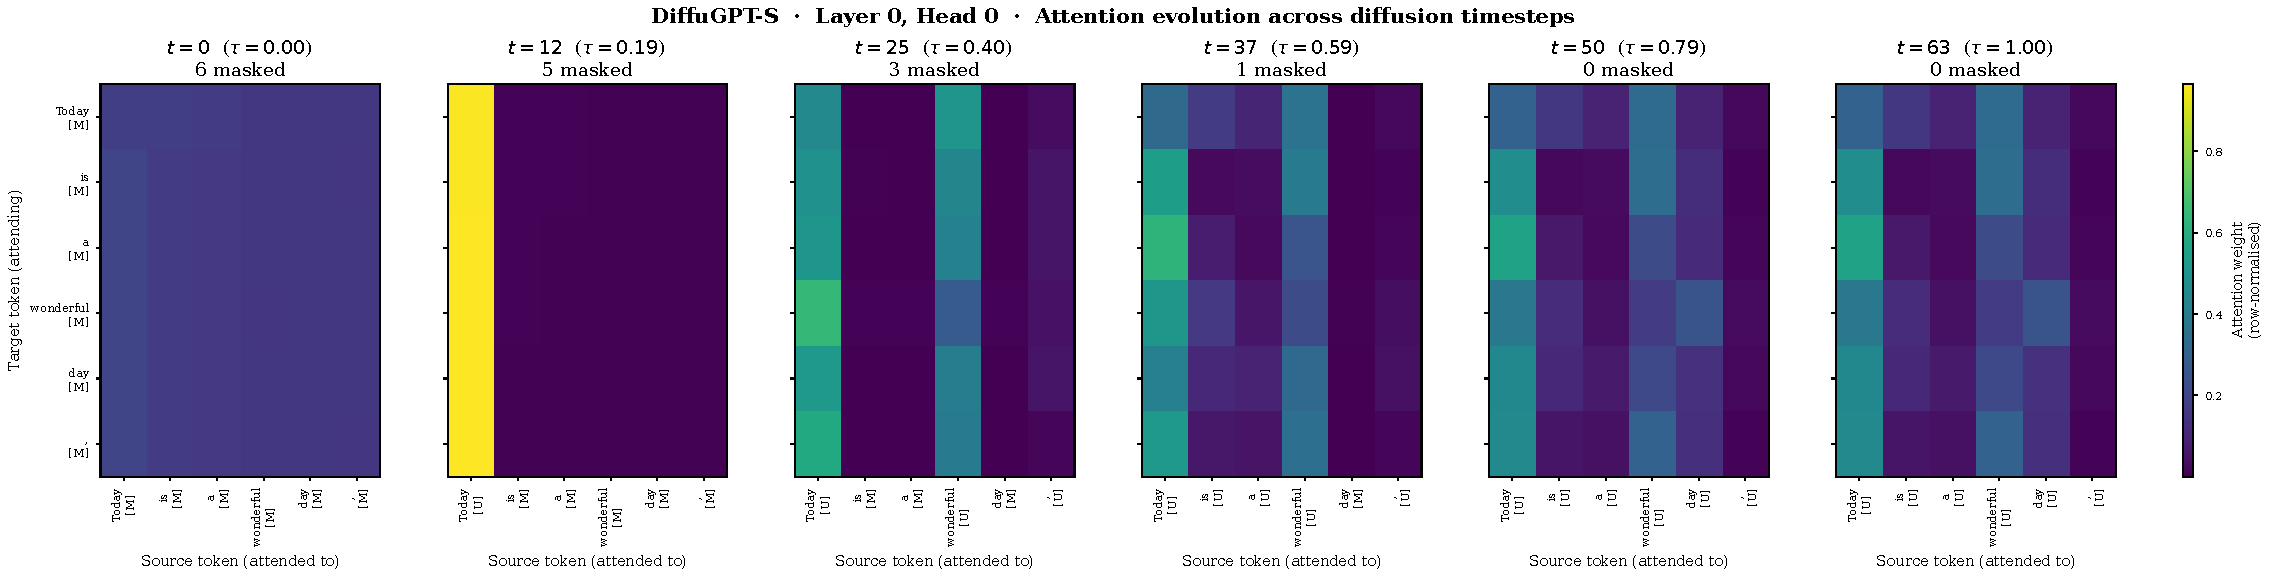
\includegraphics[width=\linewidth, height=4.5cm, keepaspectratio=false]{figures/attn_L0H0_diffusion_panel_horizontal.pdf}
    \caption{Attention heatmaps for the early-layer head (Layer~0, Head~0) at six diffusion timesteps.}
    \label{fig:l0_heatmap_5steps}
\end{subfigure}

\vspace{0.5em}

\begin{subfigure}[t]{\linewidth}
    \centering
    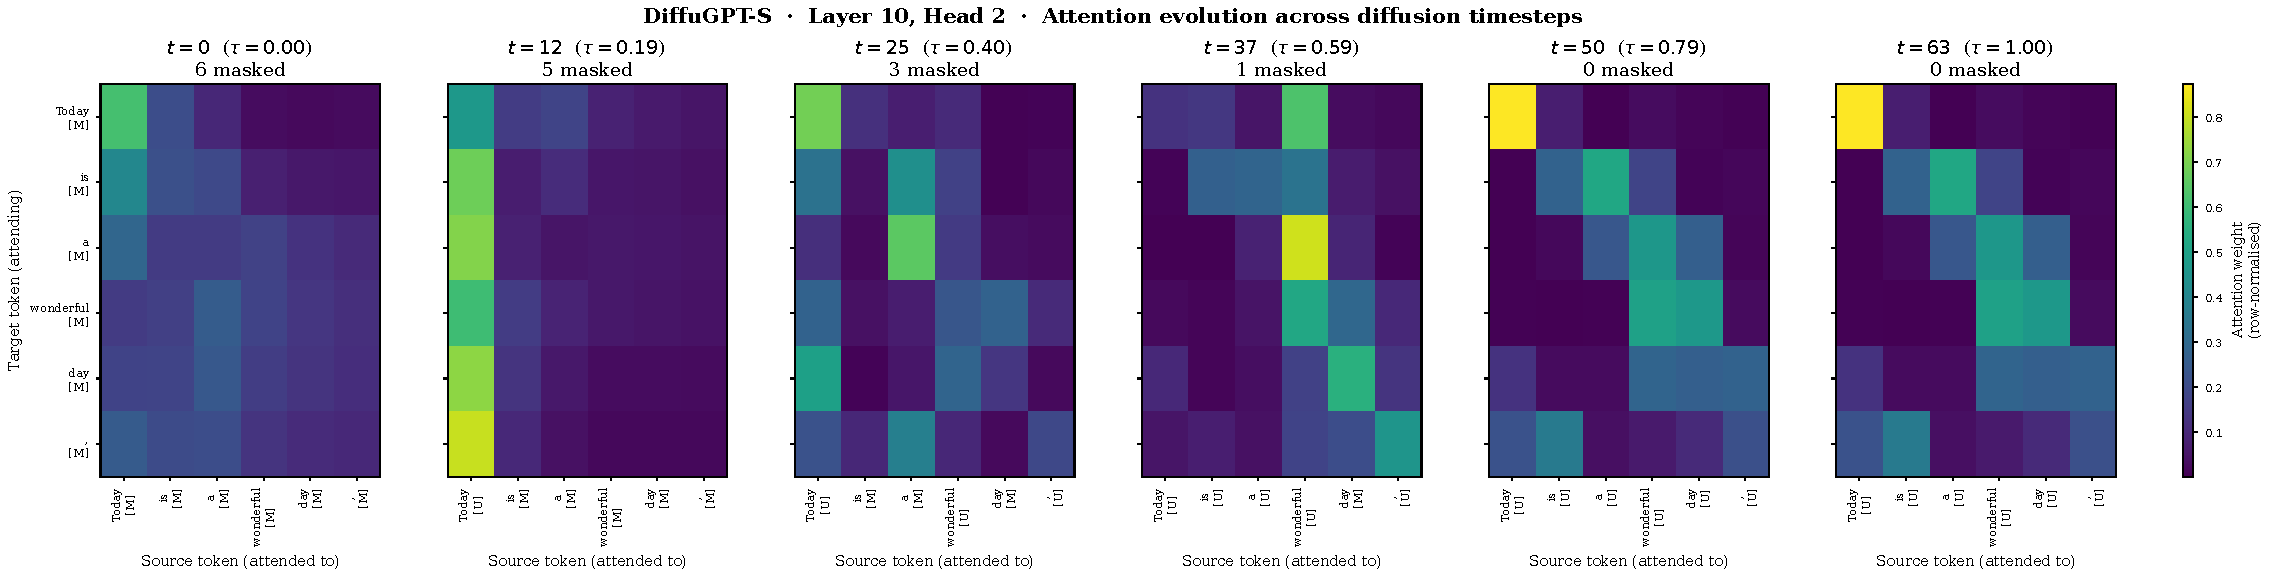
\includegraphics[width=\linewidth, height=4.5cm, keepaspectratio=false]{figures/attn_L10H2_diffusion_panel_horizontal.pdf}
    \caption{Attention heatmaps for the later-layer head (Layer~10, Head~2) at six diffusion timesteps.}
    \label{fig:l10_heatmap_5steps}
\end{subfigure}
\caption{%
Corresponding attention heatmaps at six spread diffusion timesteps for the early-layer
head~\subref{fig:l0_heatmap_5steps} and later-layer head~\subref{fig:l10_heatmap_5steps}.
Together these show that attention structure changes over denoising time and that shallow
and deep heads evolve differently.
}
\label{fig:heatmap_plots}
\end{figure}

\begin{figure}[H]
    \centering
    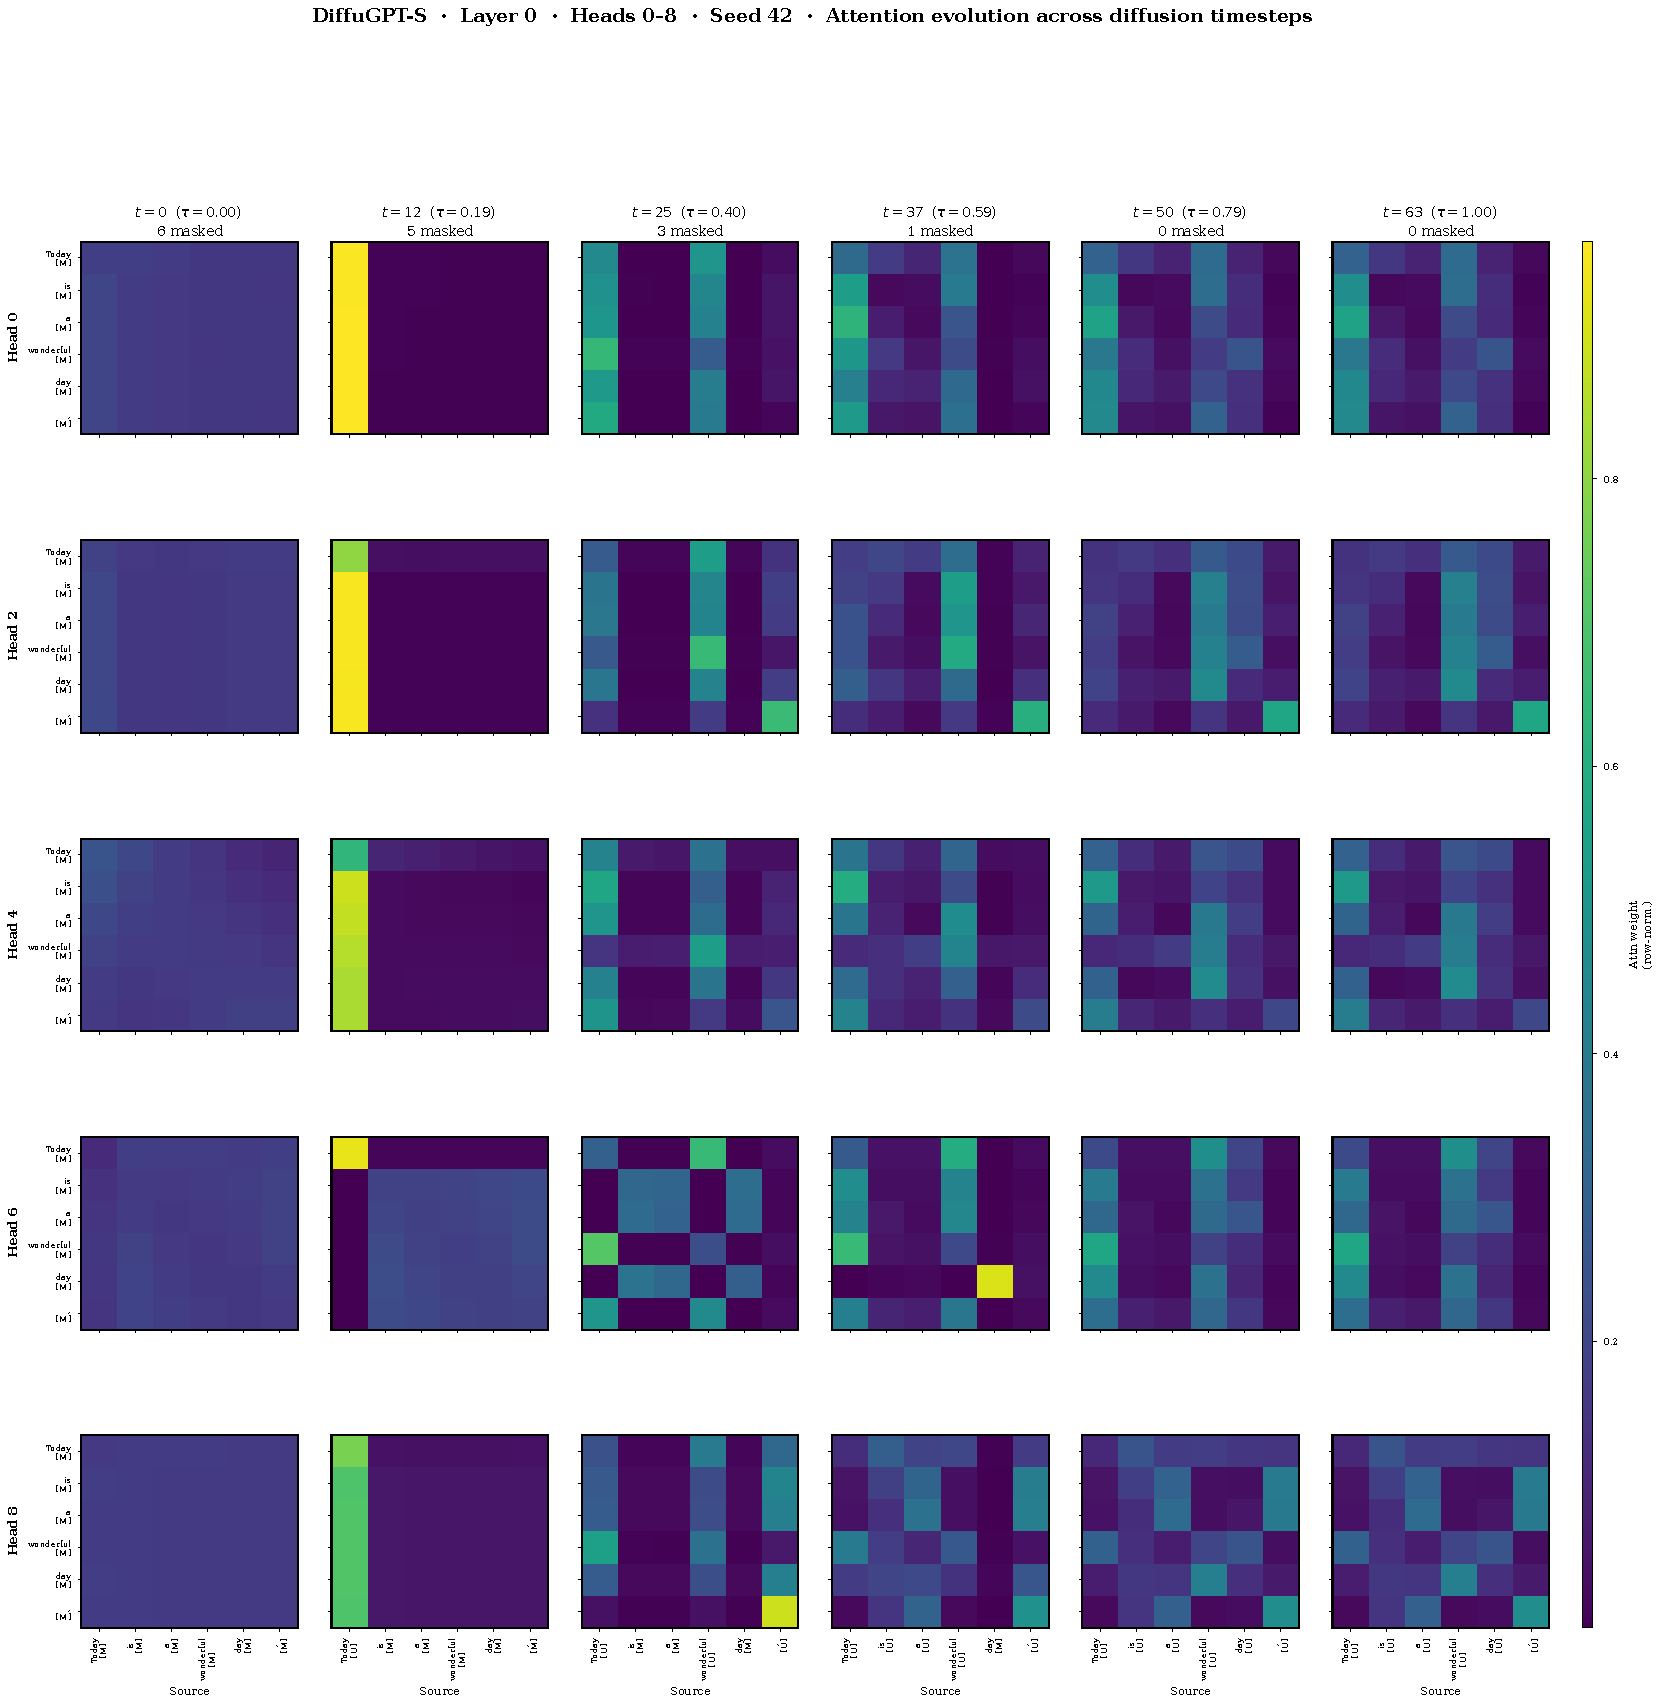
\includegraphics[scale=0.33]{figures/attn_L0_heads0-8_diffusion_panel.pdf}
    \caption{Attention evolution for Layer~0, Heads 0--8 across six diffusion timesteps.}
\end{figure}
\begin{figure}[H]
    \centering
    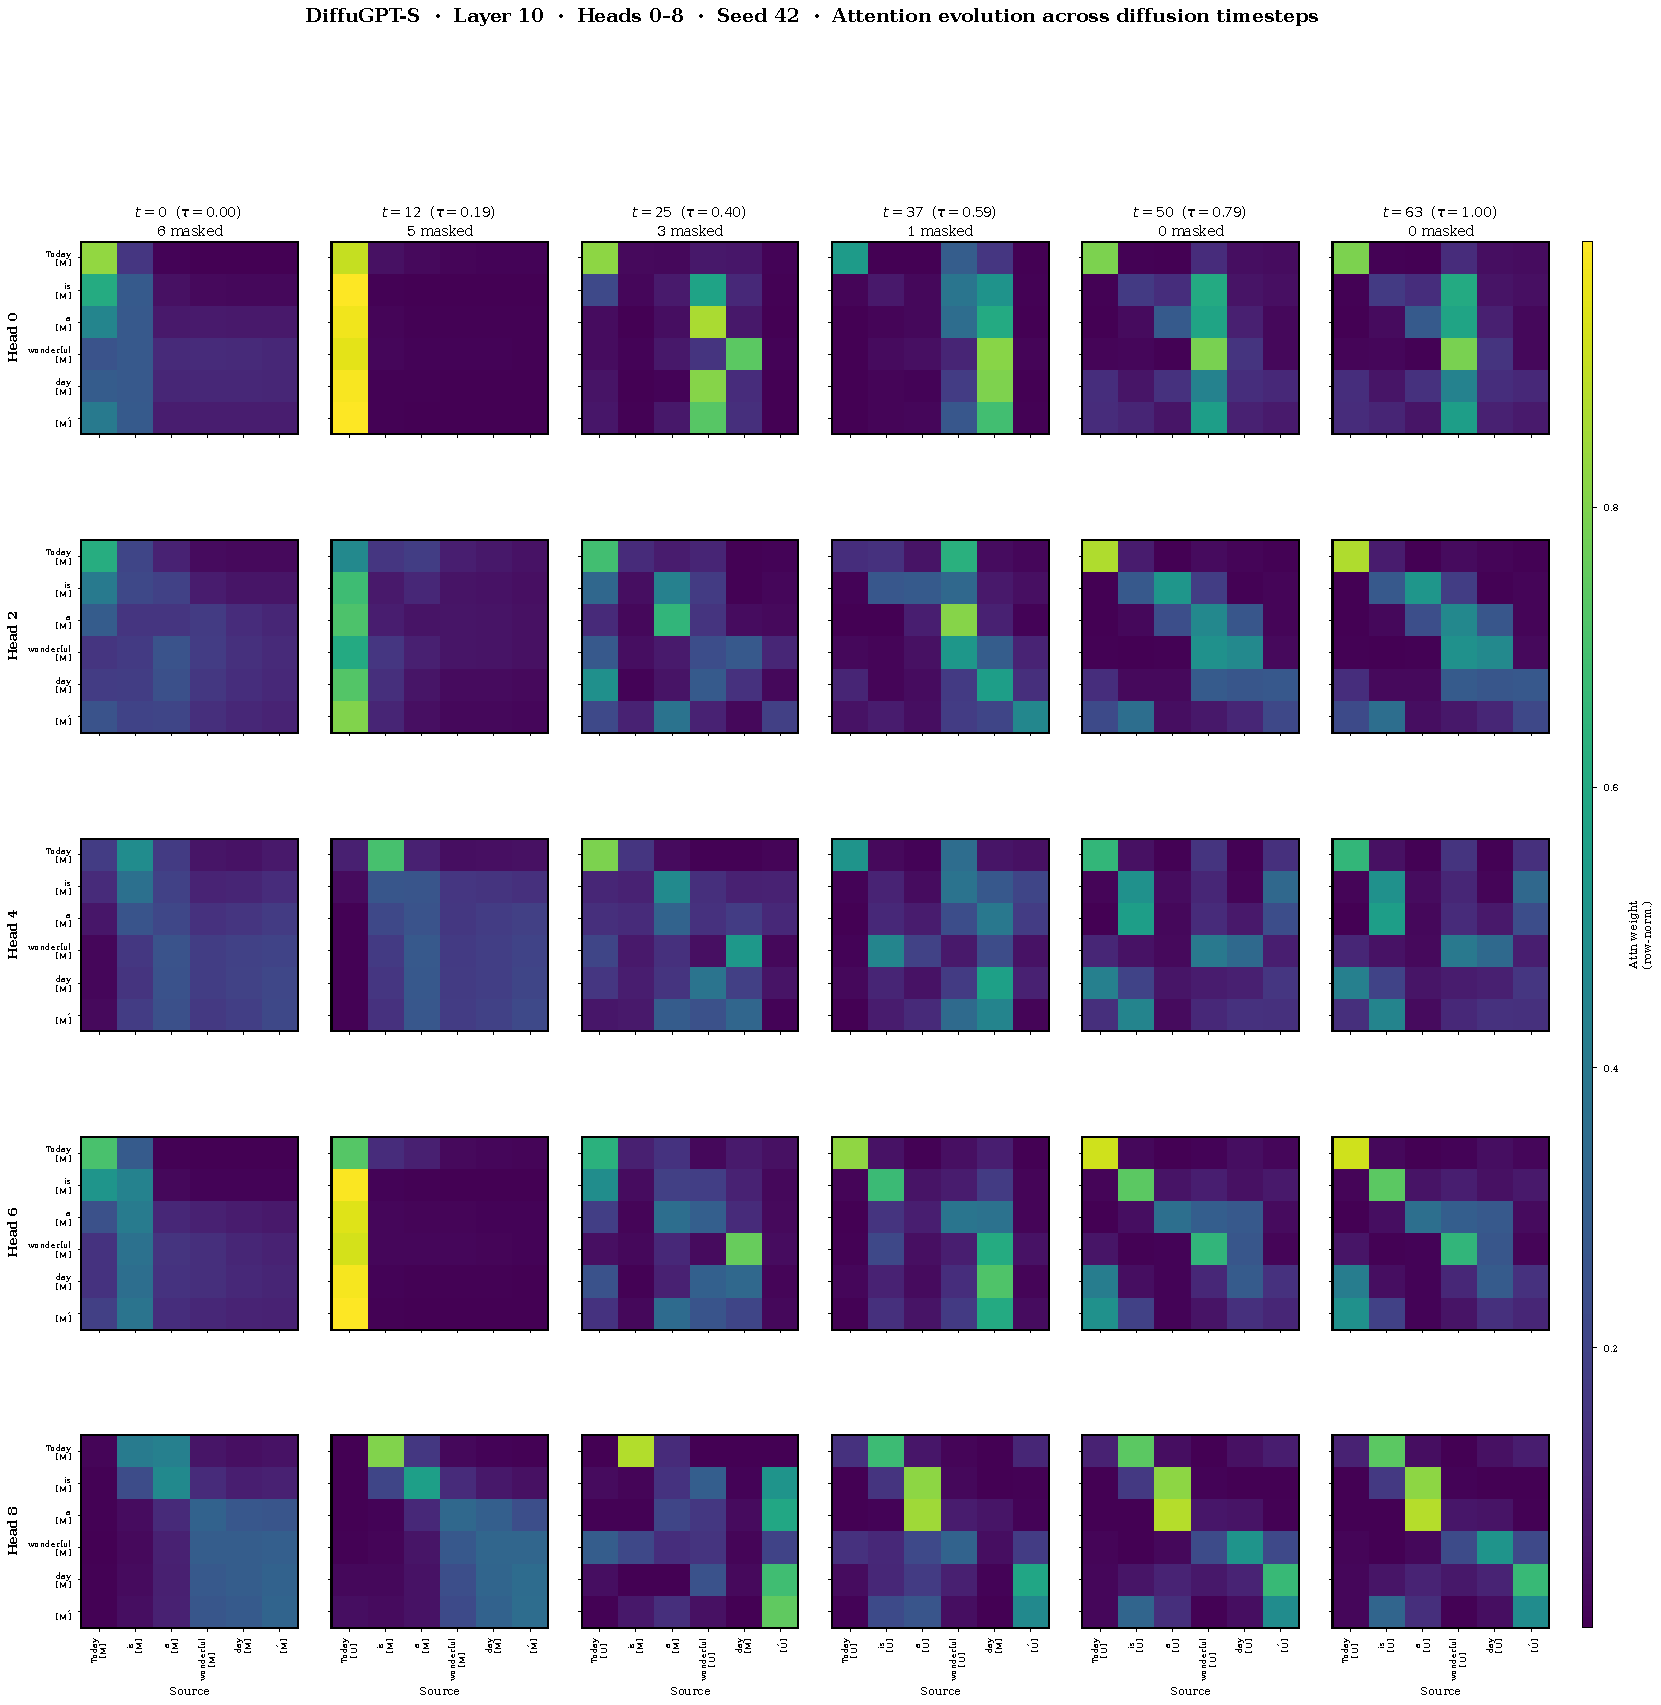
\includegraphics[scale=0.33]{figures/attn_L10_heads0-8_diffusion_panel.pdf}
    \caption{Attention evolution for Layer~10, Heads 0--8 across six diffusion timesteps.}
\end{figure}

\subsection{Attention plots}

\begin{figure}[H]
\centering
\begin{subfigure}[t]{0.49\linewidth}
    \centering
    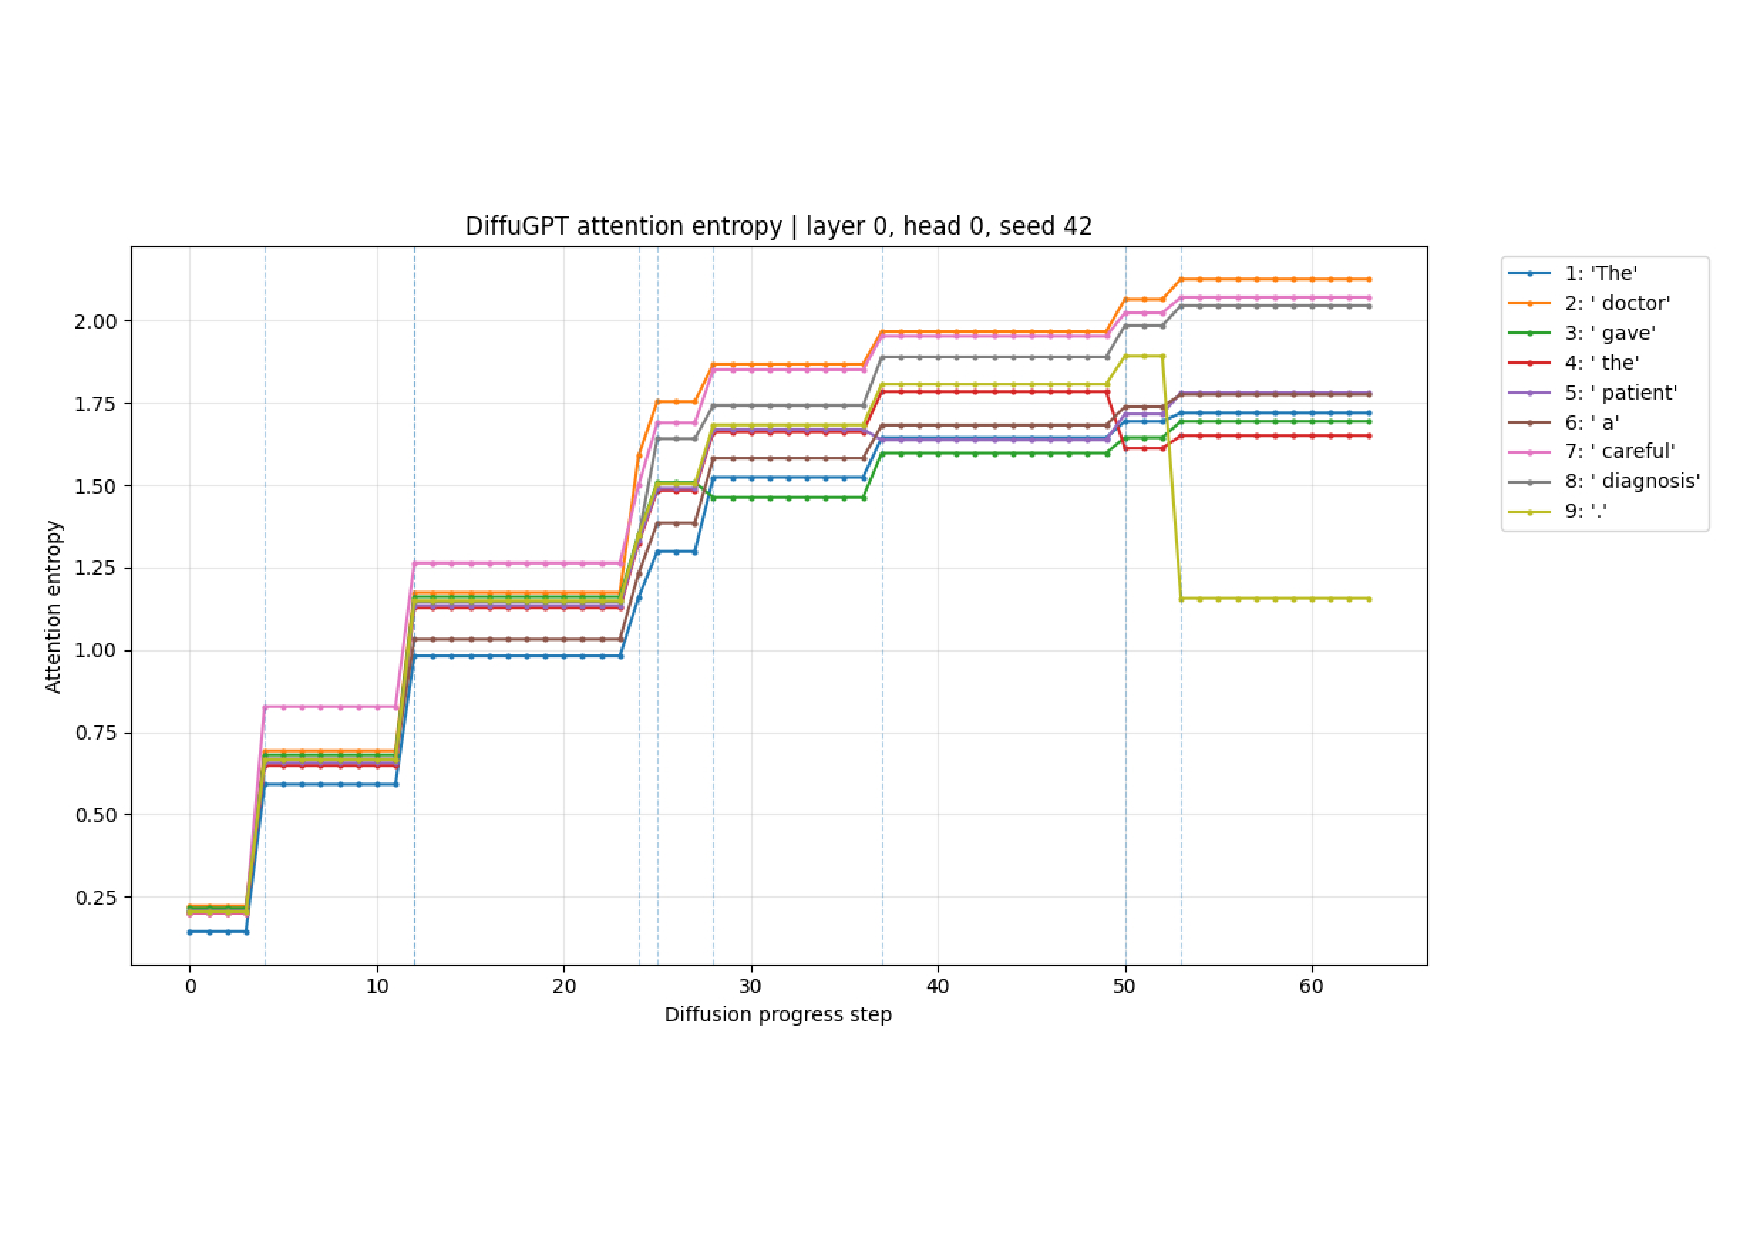
\includegraphics[width=\linewidth]{figures/attention_entropies_increasing.pdf}
    \caption{Early-layer head with increasing entropy.}
    \label{fig:l0_entropy_increase}
\end{subfigure}
\hfill
\begin{subfigure}[t]{0.49\linewidth}
    \centering
    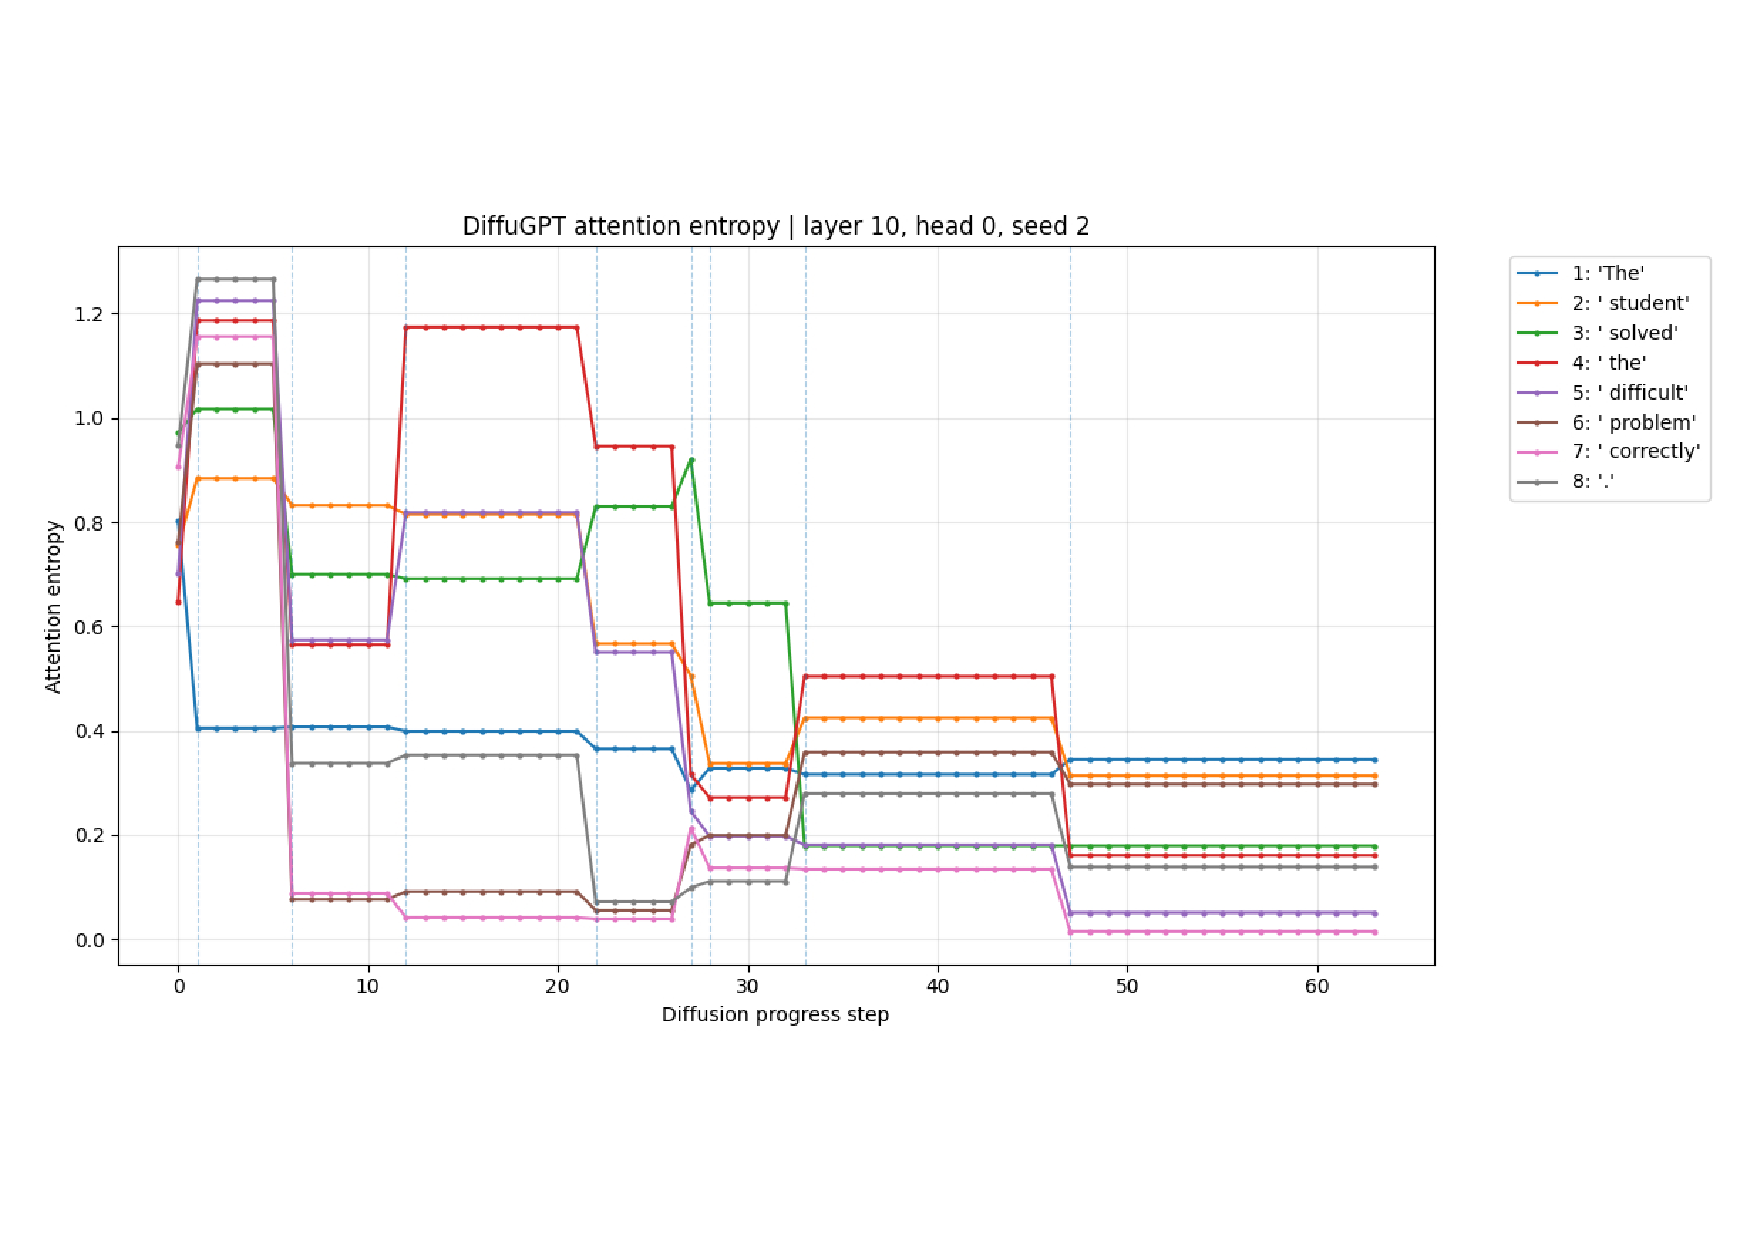
\includegraphics[width=\linewidth]{figures/attention_entropies_decreasing.pdf}
    \caption{Later-layer head with decreasing entropy.}
    \label{fig:l10_entropy_decrease}
\end{subfigure}
\caption{%
Entropy trajectories over diffusion time for an early-layer head whose attention
becomes more diffuse~\subref{fig:l0_entropy_increase} and a later-layer head whose
attention becomes more selective~\subref{fig:l10_entropy_decrease}.
}
\label{fig:entropy_plots}
\end{figure}


\subsection{Attention Patterns}
\label{app:attention_patterns}

\begin{figure}[p]
    \centering
    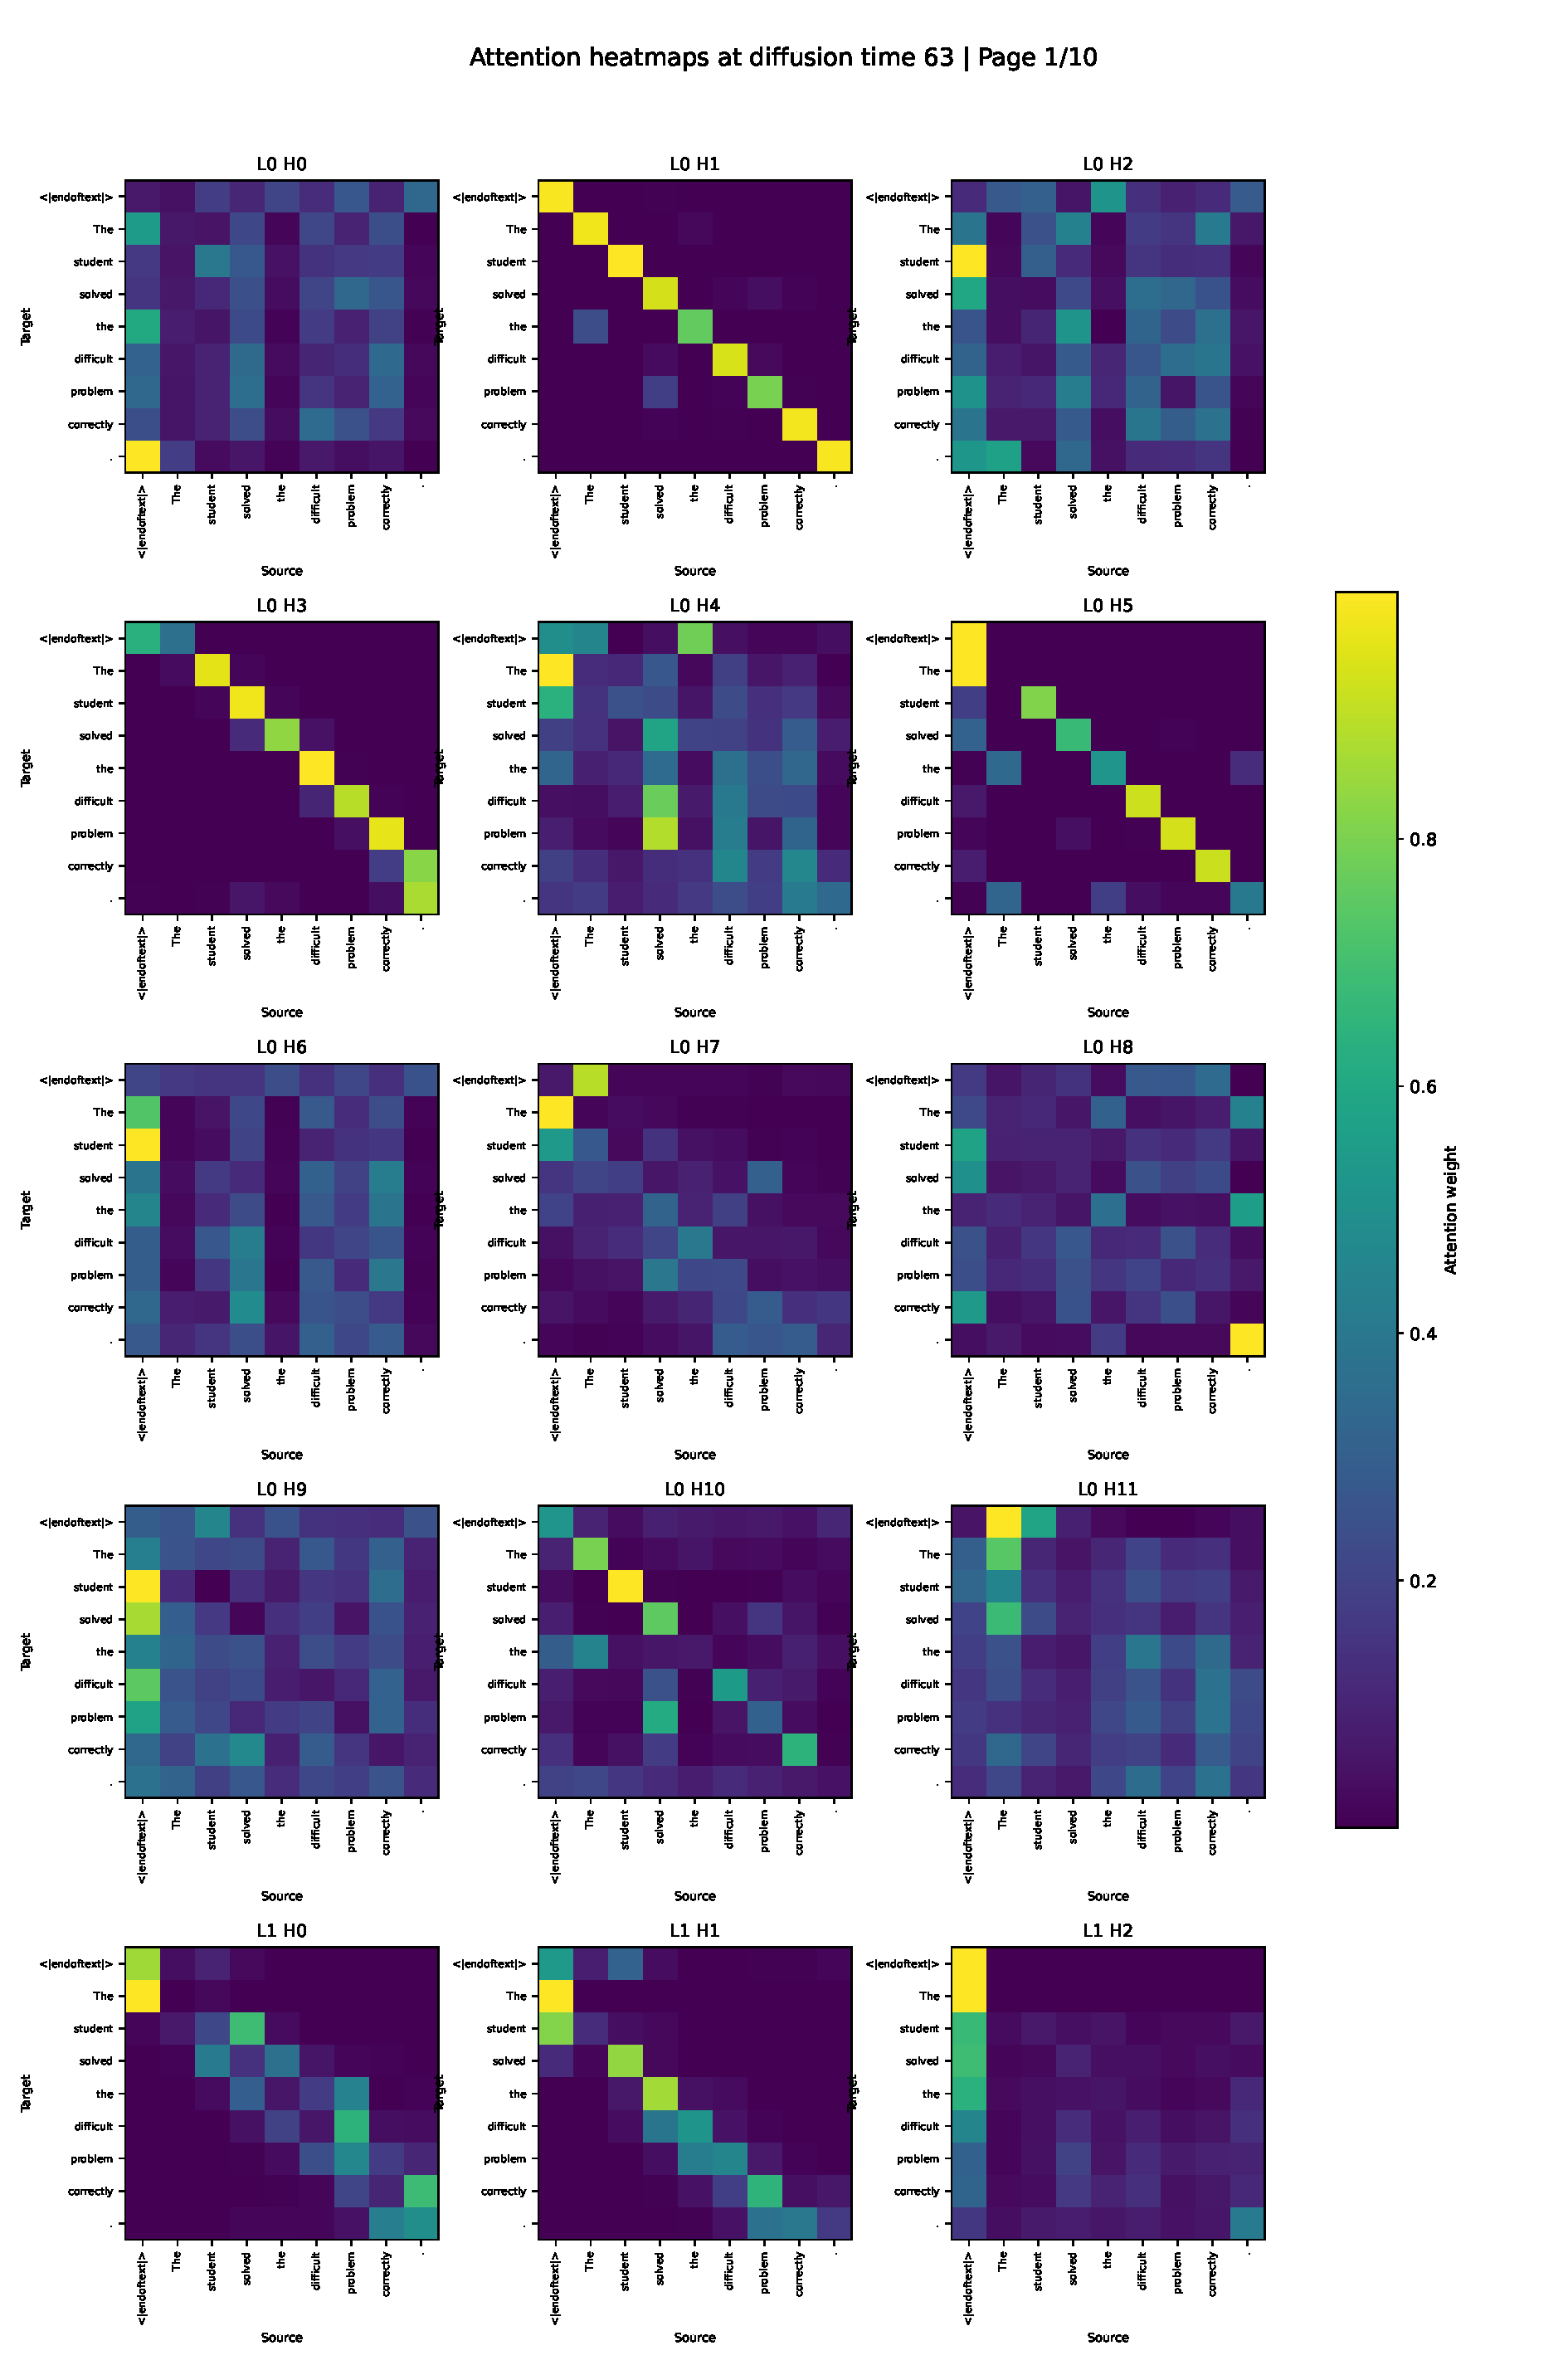
\includegraphics[scale=0.43]{figures/all_144_heads_with_bos_grid.pdf}
    \caption{Attention patterns for every head in DiffuGPT-S on a fully unmasked input sentence at diffusion time $t=63$. Notable heads include L0~H1 (self-token, self mass $\approx 0.95$), L0~H3 (next-token, $\approx 0.86$), L1~H1 (previous-token, $\approx 0.66$), and L2~H7 (punctuation, period mass $\approx 0.77$).}
    \label{fig:all_heads}
\end{figure}

\begin{figure}[H]
\centering
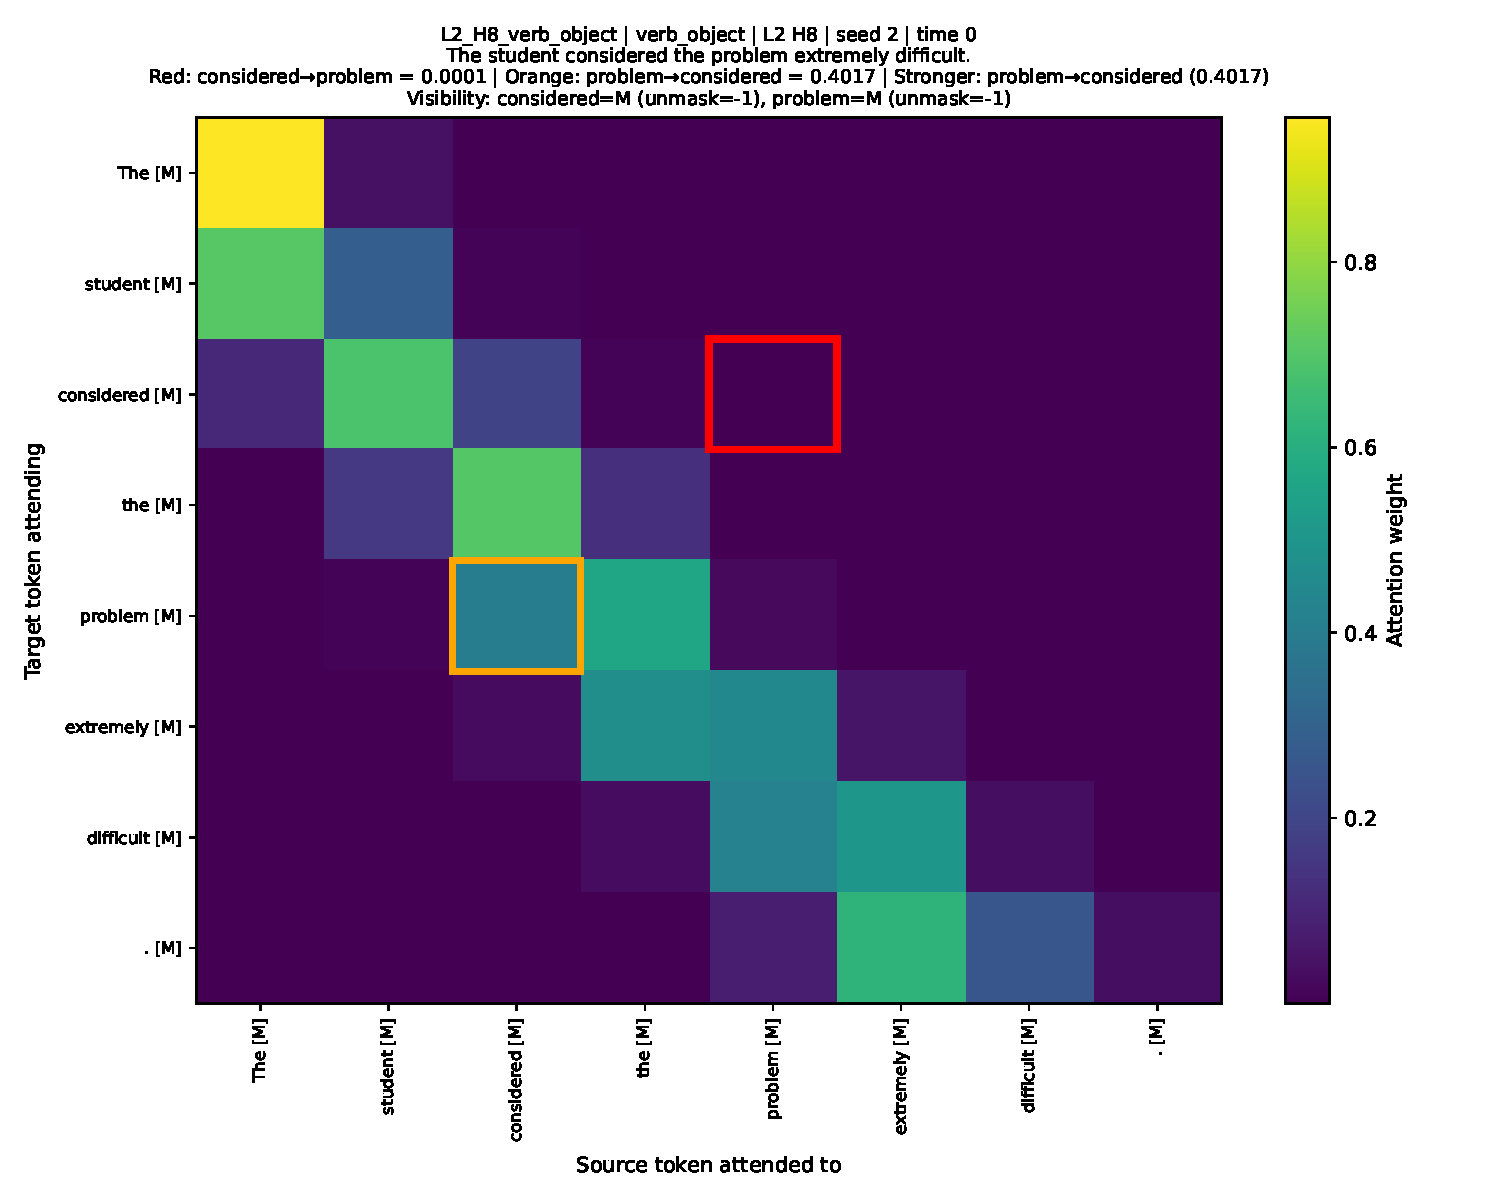
\includegraphics[width=0.82\linewidth]{figures/GLOBAL_L2_H8_verb_object_considered_problem_seed2_besttime40_The_student_considered_the_problem_.pdf}
\caption{Qualitative diagnostic heatmap for L2~H8 on an object--verb example, illustrating object$\to$verb attention at masked timesteps. This hand-selected, weight-based view is qualitative, and the held-out UD analysis (Figure~\ref{fig:ud_relation_accuracy_over_time}) provides the quantitative test across diffusion time.}
\label{fig:object-verb}
\end{figure}

\subsection{Additional Linear Probe Results}
\label{app:linear_probe_results}

This appendix presents supplementary validation and diagnostics results for the linear probe experiments from Section~\ref{subsec:shallow_class}. We show in the main text that POS/token-class information can be decoded from masked token representations. Below we present three additional tests: control baselines, intra-layer head variance in Layer~2, and ablations on the most POS-decodable heads.

\paragraph{Control baselines.}
We compare our probes to three controls---majority class, shuffled labels, and random feature probes with equal dimensionality---to rule out class-imbalance or random-feature artifacts.

\begin{table}[H]
\centering
\small
\begin{tabular}{lrrrr}
\toprule
Layer & Real probe & Majority & Shuffled labels & Random features \\
\midrule
2 & 0.920 & 0.313 & 0.250 & 0.228 \\
5 & 0.914 & 0.313 & 0.244 & 0.221 \\
10 & 0.870 & 0.313 & 0.231 & 0.216 \\
\bottomrule
\end{tabular}
\caption{Accuracy of held-out POS/token-class probes relative to control baselines. Genuine probes outperform majority-class, shuffled-label, and random-feature controls by a wide margin, demonstrating the linear decodability of token-class information from DiffuGPT-S representations.}
\label{tab:pos_probe_controls}
\end{table}

The majority-class baseline obtains $0.313$; shuffled-label and random-feature controls obtain $0.21$--$0.25$. Genuine probes obtain $0.920$, $0.914$, and $0.870$ for Layers~2, 5, and 10 respectively.

\paragraph{Head-level variation.}
To test whether POS information is equally decodable from each attention head within a layer, we run head-level probing experiments on Layer~2.

\begin{figure}[H]
\centering
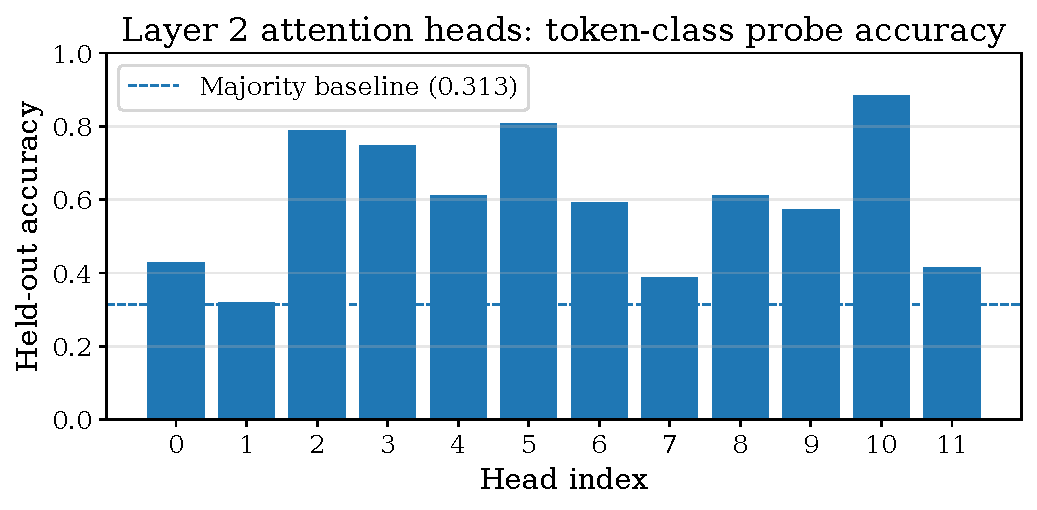
\includegraphics[scale=0.5]{figures/layer2_head_token_class_accuracy.pdf}
\caption{Head-level POS/token-class probe accuracy in Layer~2. Token-class information is not equally decodable from all heads; some heads are significantly more accurate than others and than the majority baseline.}
\label{fig:layer2_head_token_class}
\end{figure}

Performance is uneven across heads: some decode POS/token-class information accurately while others are near the majority baseline, indicating that POS information is not uniformly distributed across attention components in Layer~2.

\paragraph{Ablation of POS-decodable heads.}
We investigate whether the most POS-decodable heads are causally necessary for maintaining token-class information. In each layer, we ablate the heads with the highest POS decodability and compare the accuracy drop against ablating less-decodable control heads.

\begin{figure}[H]
\centering
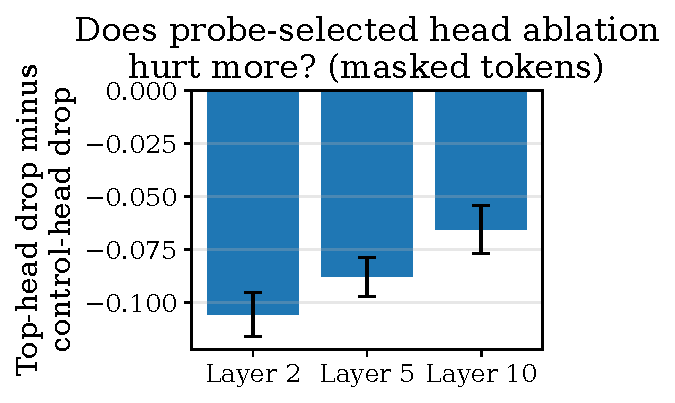
\includegraphics[width=0.7\linewidth]{figures/top_minus_control_effect_masked.pdf}
\caption{Effect of ablating the most POS-decodable heads vs.\ less-decodable control heads on masked-token POS accuracy. Negative or near-zero values indicate that the most decodable heads are not the causally most important heads for preserving token-class information.}
\label{fig:pos_ablation_top_minus_control}
\end{figure}

Ablating the most POS-decodable heads does not produce a greater accuracy drop than ablating the control heads. This contradicts the simplest causal interpretation of the probe findings: while POS information is linearly readable from certain heads, the model does not causally depend on those specific heads.

\section{Prediction Before Unmasking: Timing Analysis}
\label{app:timing}

\begin{figure}[t]
\centering
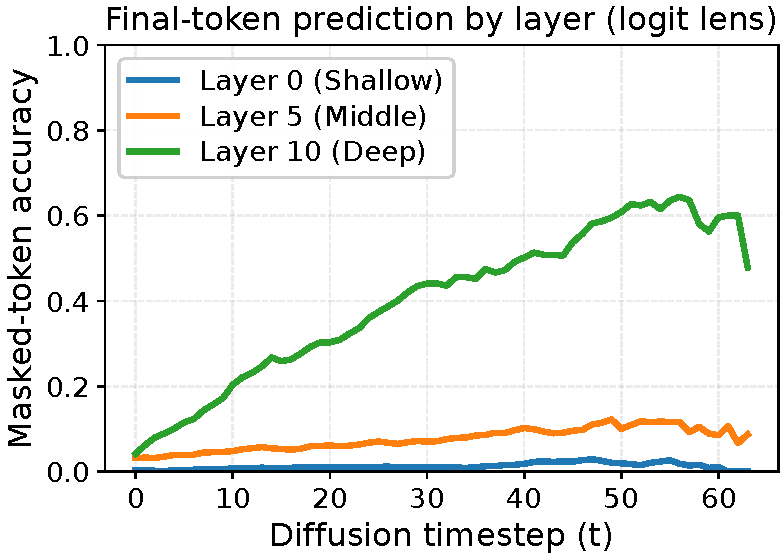
\includegraphics[scale=0.42]{figures/final_token_prediction.pdf}
\caption{Masked-token identity accuracy of a per-layer logit lens over diffusion
time. Deeper layers decode the eventual token far better than shallow layers.}
\label{fig:final_token_prediction}
\end{figure}


This appendix details the timing analysis summarized in Section~\ref{subsec:deep_identity}: when, over the course of denoising, the model commits to the token a masked position will eventually take. We generate diffusion trajectories for \texttt{diffugpt-s} on $24$ prompts ($12$ reasoning, $12$ creative) with $64$ diffusion steps and a generation length of $96$, and for each generated position record its found time $f_i$ (the first step at which the final-layer argmax equals the eventual token) and unmmask time $u_i$ (the first step at which the position is revealed as that token).

DiffuGPT-S does not reveal tokens greedily: at each step it samples the revealed token from a top-$p$ ($p{=}0.9$), temperature-scaled ($T{=}0.95$) distribution and randomly selects which masked positions to reveal with probability $1/(t{+}1)$. Across $1{,}743$ unmasking events, the revealed token matches the model's own final-layer argmax at the preceding step only $50.1\%$ of the time. This stochasticity bounds how well any representation can predict the exact realized token at the moment of unmasking, so the depth-wise identity results in Section~\ref{subsec:deep_identity} are conservative and would be expected to sharpen under greedy decoding.

Averaging, at each diffusion step, the fraction of generated positions whose final-layer argmax already equals the eventual token, the correct-prediction fraction rises smoothly and approximately linearly from about $0.05$ to a plateau of $0.772$ for reasoning prompts and $0.739$ for creative prompts. Reasoning reaches half of its final correctness at diffusion progress $0.40$ and $90\%$ at $0.90$; creative reaches the same milestones slightly earlier, at $0.38$ and $0.84$. Refinement is therefore steady rather than concentrated in a single burst, and the two task types behave similarly.

Of $1{,}613$ positions with a valid measurement, $63.4\%$ are predicted before they are unmasked ($f_i < u_i$), by a mean of $9.0$ and a median of $7.0$ diffusion steps, up to a maximum lead of $63$ steps---essentially the entire trajectory; a further $10.4\%$ are predicted exactly at the unmask step. The per-token lead distribution is strongly skewed toward early prediction, with a spike at zero and a heavy tail of positions committed tens of steps in advance. Early commitment is concentrated in structural tokens: $61\%$ of punctuation positions and $54\%$ of function-word positions are predicted early, compared with $44\%$ of content-word positions, indicating that the model fixes syntactic scaffolding before resolving content words.

\section{Linguistic Relation Heads: Attribution and Ablation}
\label{app:relation_heads}

This appendix provides the detailed evidence behind the relation-head analysis of Section~\ref{subsec:attn_patterns}. Using diagnostic sentences with known relation pairs (subject--verb, verb--object, adjective--noun), we (i) recover recognizable surface-pattern heads at the final step, (ii) show that relation-token attention is present while the tokens are still masked, (iii) measure with Direct Logit Attribution whether the relevant heads write support for the eventual token, and (iv) test this causally with matched ablations.

\subsection{Surface-Pattern Heads}
At the final, fully unmasked step several heads implement simple positional patterns, confirming that the heatmap method recovers known motifs before we search for higher-level relations: Layer~0 Head~1 is a self-token head (self mass $\approx 0.95$), L0~H3 a next-token head ($\approx 0.86$), L1~H1 a previous-token head ($\approx 0.66$), and L2~H7 a punctuation head (period mass $\approx 0.77$). The full $144$-head grid is shown in Figure~\ref{fig:all_heads}.

\subsection{Relation Attention at Masked Positions}
For a labeled token pair we define the relation attention score as the larger of the two directional attention weights, the dominant direction as the corresponding direction, and the consistency fraction as the proportion of controlled sentences in which the dominant direction agrees.

\paragraph{Verb--object (L2~H8).} Across five controlled sentences, L2~H8 has mean relation score $0.648$, consistency $1.0$, and dominant direction object$\to$verb (per sentence: problem$\to$solved $0.969$, patient$\to$examined $0.547$, lesson$\to$explained $0.382$, match$\to$won $0.873$, result$\to$studied $0.468$). On ``The student considered the problem extremely difficult'' (seed~2), the edge problem$\to$considered measures $0.40$, $0.60$, $0.37$, and $0.24$ at diffusion times $0,5,10,20$, with both tokens masked throughout.

\paragraph{Subject--verb (L5~H0, L8~H6).} L5~H0 has mean subject--verb score $0.909$, consistency $1.0$, and dominant direction subject$\to$verb. On ``The doctor carefully examined the sick patient'' (seed~1), L8~H6 shows doctor$\to$examined $=0.993$ at time~$10$ while both tokens are masked.

\paragraph{Non-adjacent adjective--noun (L2~H10).} On ``The problem that seemed difficult confused the student,'' L2~H10 shows difficult$\to$problem $=0.899$ at time~$20$ (vs.\ problem$\to$difficult $=0.003$) with both tokens masked, and $0.636$ already at time~$5$. Because the two tokens are not adjacent, this is unlikely to reflect a previous-/next-token heuristic.

\subsection{Direct Logit Attribution}
We apply Direct Logit Attribution (Section~\ref{subsec:dta}) to test whether these heads write support for the eventual token, reporting the target token's vocabulary percentile under the head's output (treating $>0.90$ as strong exact-token evidence) alongside its token-type attribution. On ``The student solved the problem yesterday'' (target \texttt{problem}, masked, times $30$/$40$), L2~H8 ranks first in relation attention ($0.894$) and places the target at vocabulary percentile $0.954$. L2~H10 (target \texttt{problem}, time~$20$) ranks first in relation attention ($0.666$) and also exceeds the $0.90$ threshold. In contrast, the subject--verb heads attend strongly (L5~H0 $0.994$, L8~H6 $0.993$) but their exact-token percentiles fall below $0.90$ (e.g.\ $0.818$ for L8~H6) while ranking highest on verb-type attribution; they are therefore best described as token-type/structural heads rather than exact-token heads.

\subsection{Causal Ablation with Matched Controls}
We zero a head's contribution and measure the change in the target-token logit. Because ablating any head perturbs the prediction---a low-relation control, L0~H0, lowers the \texttt{problem} logit by $-1.33$ despite negligible relation attention ($0.002$)---we compare each relation head against multiple low-relation control heads on the same sentence, target, seed, and timestep. The reported statistic is the fraction of controls whose target-logit drop is at least as large as the relation head's; lower values indicate stronger relation-specific evidence (Table~\ref{tab:mini_control_ablation}).

\begin{table}[H]
\centering
\small
\resizebox{\linewidth}{!}{
\begin{tabular}{llrrrr}
\toprule
Case & Head & Winner $\Delta$ logit & Control mean & Gap & Controls $\geq$ winner \\
\midrule
L2H10 adj--noun & L2 H10 & -1.558542 & -0.076344 & -1.482198 & 0\% \\
L2H8 verb--object & L2 H8 & -0.255547 & 0.023125 & -0.278672 & 8.33\% \\
L5H0 subj--verb & L5 H0 & -0.169333 & 0.305876 & -0.475209 & 8.33\% \\
\bottomrule
\end{tabular}
}
\caption{Causal ablation results comparing selected high-relation heads against low-relation control heads. ``Controls $\geq$ winner'' reports the fraction of control heads whose target-logit drop was at least as negative as the selected head's drop. Lower values indicate stronger relation-specific causal evidence.}
\label{tab:mini_control_ablation}
\end{table}

Across all three cases the relation head reduces target-token support more than the typical low-relation control, which is consistent with relation-specific causal effects rather than generic ablation damage. We stress that three hand-inspected cases cannot establish this in general; a population-level ablation over the full held-out set is left to future work. The combined visual, attribution, and causal evidence is strongest for L2~H10 (non-adjacent adjective--noun) and L2~H8 (verb--object); L5~H0 provides structural/causal subject--verb evidence, whereas L8~H6 shows strong relation attention but weaker attribution and a negligible ablation effect ($\Delta$ logit $-0.013$). No single head determines the eventual token: relation heads provide measurable relation-specific support while final-token prediction remains distributed across heads, layers, and later computation.

\subsubsection*{Acknowledgments}
% TODO: Add funding acknowledgments here before camera-ready submission.

\end{document}